\chapter{Introduction}

\section{Quantum Chromodynamics}

Quantum Chromodynamics (QCD) is the fundamental theory of the strong force and describes the interactions between quarks which is mediated by gluons. Quarks come in 6 flavors: up, down, strange, charm, bottom, and top. All quarks have a fractional electric charge (either $\pm \frac{1}{3}e$ or $\pm \frac{2}{3}e$). Quarks carry a color (red, green, or blue) and are bound by gluons into groups of three (baryons) or two (mesons). Baryons and mesons have no color, in baryons the three colors add up in a way that is color neutral while in mesons the one quark carries a color and the antiquark carries a corresponding anticolor. 

Deep inelastic scattering (DIS) experiments at SLAC first revealed the structure of nucleons and showed that they were composed of three spin-$1/2$ particles. These measurements confirmed the quark model and showed that quarks were real particles within hadrons. DIS experiments also suggested other peculiar and (at the time) unexpected behaviors in quarks. When bound quarks are probed at higher energy scales they behave as if they were free. In fact it is the case with quarks that with large momentum exchange the coupling between quarks and gluons is weak and we can treat QCD perturbatively. However as the energy scale decreases the coupling becomes stronger and perturbation theory no longer applies. This property of QCD is called asymptotic freedom and was discovered in 1973 by Gross, Wilczek, and Politzer for which they were awarded the Nobel Prize in 2004. Asymptotic freedom arises in QCD because it is a non-Abelian gauge theory. There is screening of the color charge of quarks by the vacuum, however there is also anti-screening from charged spin-1 gluons. The value of the coupling in QCD can be represented by the $\beta$ function, for QCD it can be shown that to lowest order $\beta(g)$ is propotional to $-(\frac{11}{2} - \frac{n}{3})$ where n is the number of quarks. For QCD, with 8 gluons and 3 colors, the anti-screening from the gluons overcomes the screening of the quarks and thus the theory is asyptotically free. Figure~\ref{fig:a_free} shows experimental estimates of $\alpha_S$ as a function of the scale of the momentum exchange. The experimental results are in agreement with the predictions of asymptotic freedom. 

\begin{figure}[htbp]
\begin{center}
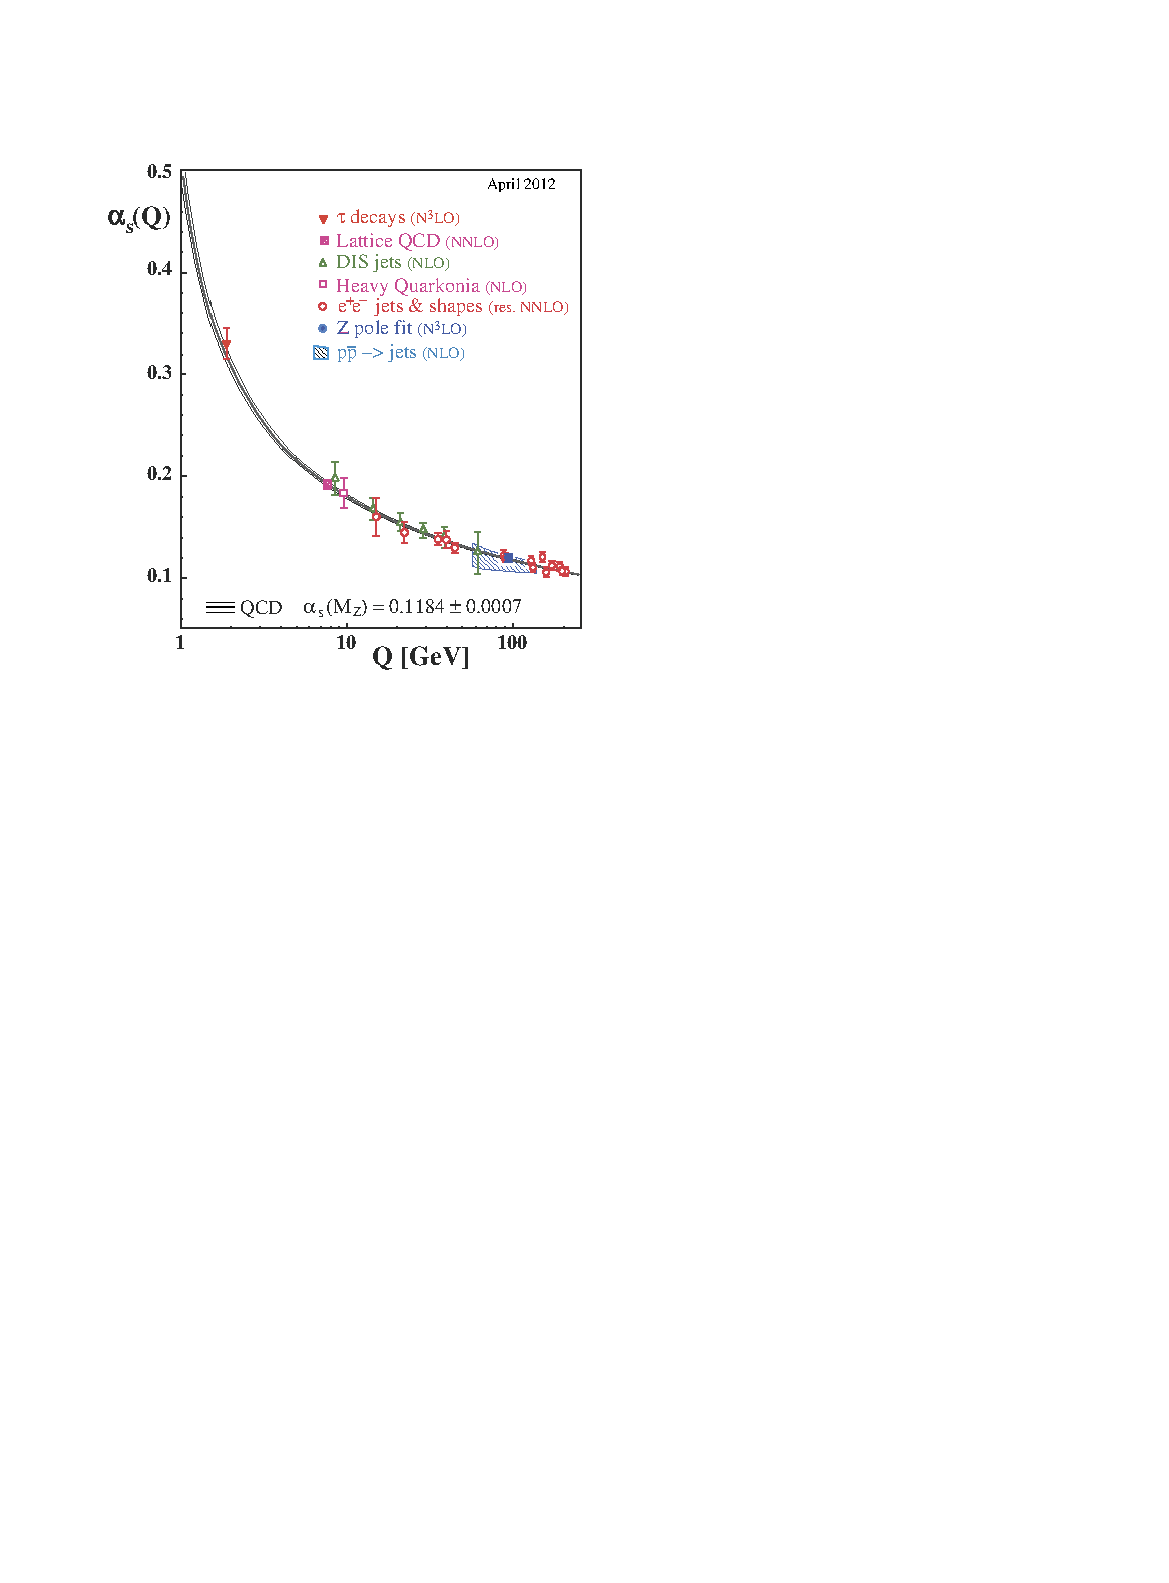
\includegraphics[scale=1.3]{Plots/Intro/asymp_free.pdf}
\end{center}
\caption[Asymptotic Freedom]{Several measurements of the strong coupling constant $\alpha_S$ showing how it varies with energy scale. Decreasing coupling strength as the interaction energy goes up is consistent with predictions of asymptotic freedom~\cite{wsalpha}.}
\label{fig:a_free}
\end{figure}

Within baryons and mesons quarks are bound in colorless states, as explained above, and at short distance scales the coupling between the quarks and gluons is weak and we can treat the interaction of quarks perturbatively. However, when we attempt to remove a quark from a hadron, lattice QCD calculations show the potential increases approximately linearly with distance. Eventually the energy put into this hypothetical system increases to a high enough point that a new quark anti-quark pair is created from the vacuum and we end up with two hadrons. This property of QCD, that quarks and gluons remain bound in colorless states, we refer to as confinement. 

Confinement and asymptotic freedom are two of the most interesting properties associated with QCD, and are responsible for many of the interesting phenomena within the strong interaction. We will next explore the QCD phase diagram, and look for evidence of confinement being broken.  

\section{QCD Phase Diagram and Deconfinement}

At low temperatures lattice calculations show that quarks are confined within hadrons, we will now turn our attention to the properties of quark matter under more extreme conditions. Lattice calculations also predict a rich phase structure in QCD beyond what we observe in low temperature hadronic matter. As we increase the temperature and density of nuclear matter it is predicted that quarks and gluons are deconfined from their hadronic states. We call this hot dense state of matter with deconfined quarks and gluons the Quark Gluon Plasma (QGP). Conditions in the universe allowed for QGP to exist up until about $10^{-5}$ s after the Big Bang. There is also the possibility that colder deconfined matter could exist within neutron stars.

Figure~\ref{fig:qcd_phase} shows an illustration of the QCD phase diagram. Nuclear matter exists in the lower right part of the figure, inside nuclei the temperatures are low and the average net baryon number is high. The figure also shows the regions of the phase diagram which are accesible to various collider and fixed-target experiements which we will discuss further in upcoming sections. Also of note is that the phase transition from QGP to hadronic matter can be a smooth cross-over and that there is postulated to be a first order phase transition in the QCD phase diagram. The search for a QCD critical point is an area of active research, but is beyond the scope of this dissertation. 

\begin{figure}[htbp]
\begin{center}
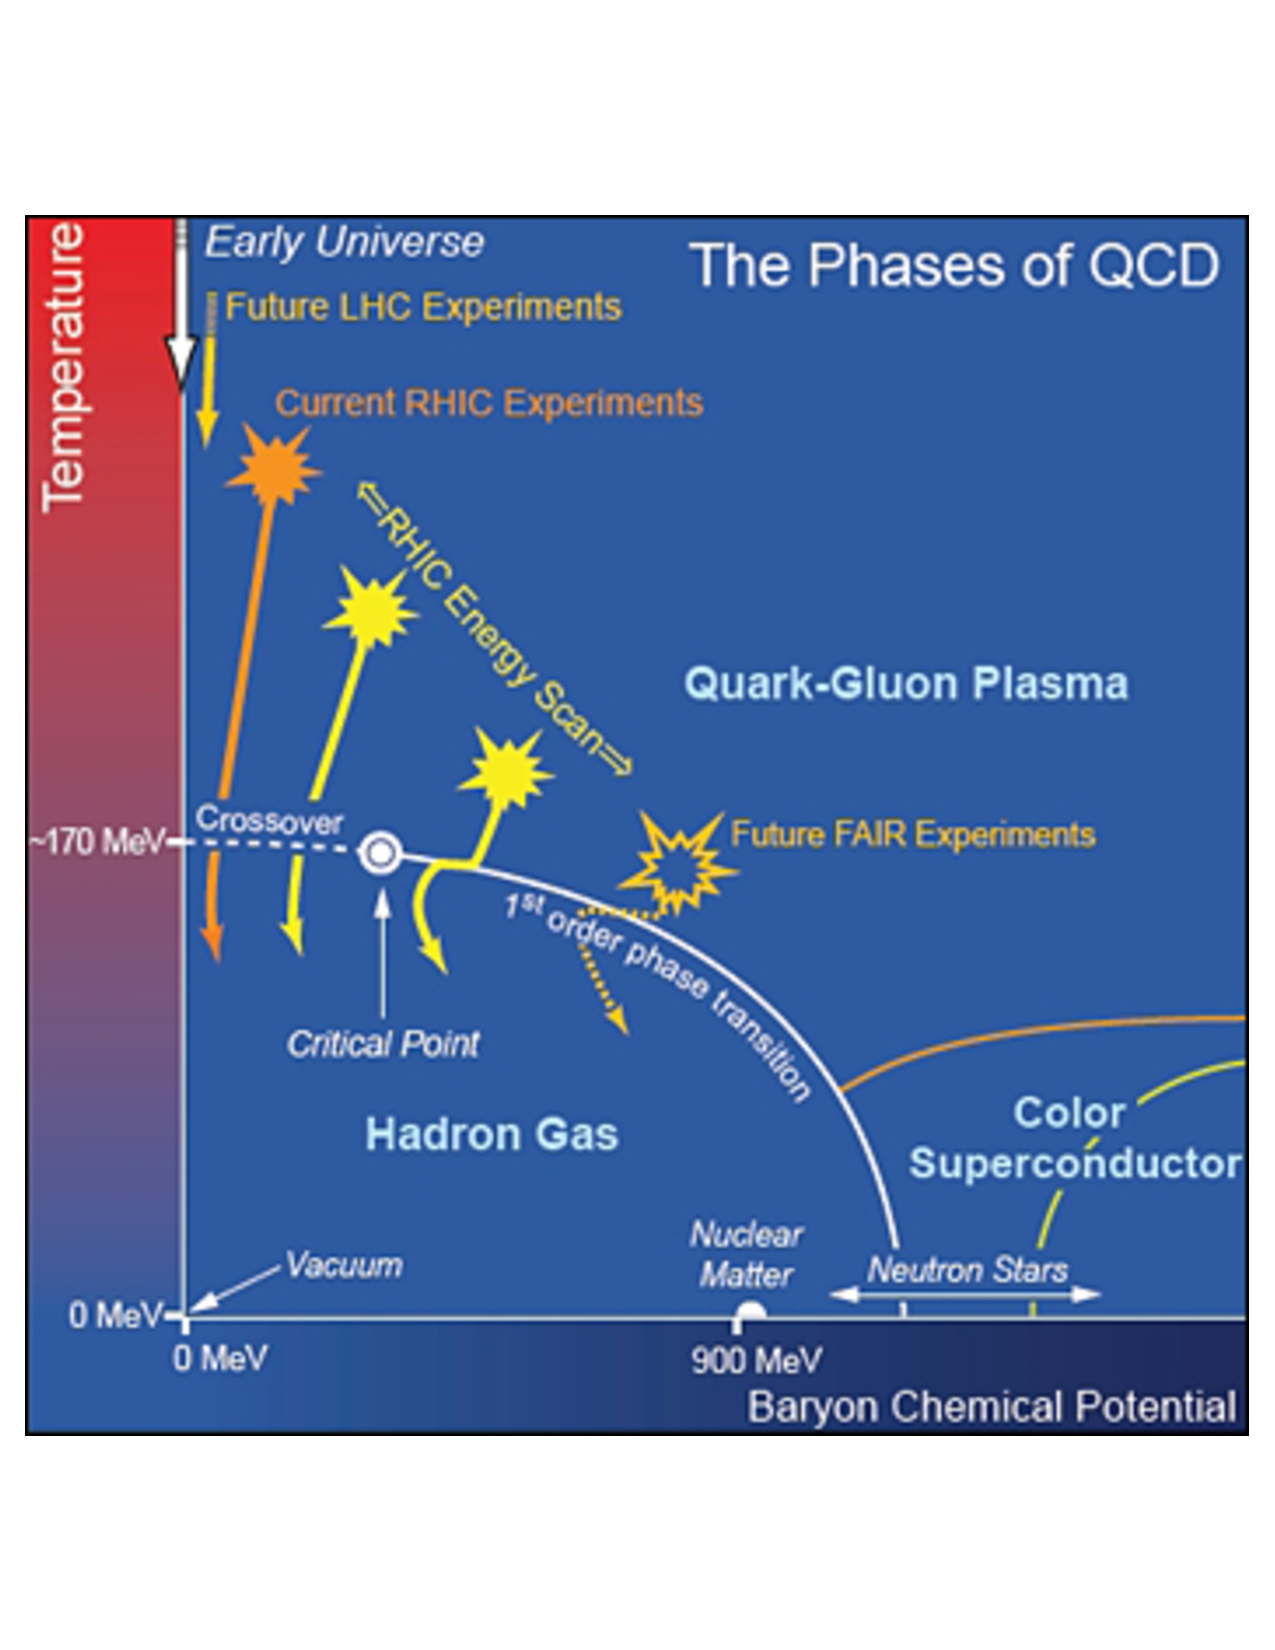
\includegraphics[scale=0.5]{Plots/Intro/qcd_phase.pdf}
\end{center}
\caption[QCD Phase Diagram]{Illustration of the QCD phase diagram showing the various regimes as well as the reach of current experiments.}
\label{fig:qcd_phase}
\end{figure}

The critical behavior can be seen in the bulk thermodynamic properties of QGP around the critical temperature $T_c$. Figure~\ref{fig:pressure} shows lattice QCD calculations of the quantity $p/T^4$ as a function of temperature for various quark flavor combinations. At the critical temperature there is a transition from hadronic to partonic degrees of freedom which is seen in the large jump in $p$~\cite{hitempQCD}. At high temperatures the medium's behavior asymptotically approaches that of an ideal gas. The increase in degrees of freedom is taken as evidence that the phase transition in QCD coincides with the onset of deconfinement and the switch from hadronic to partonic degrees of freedom.

\begin{figure}[htbp]
\begin{center}
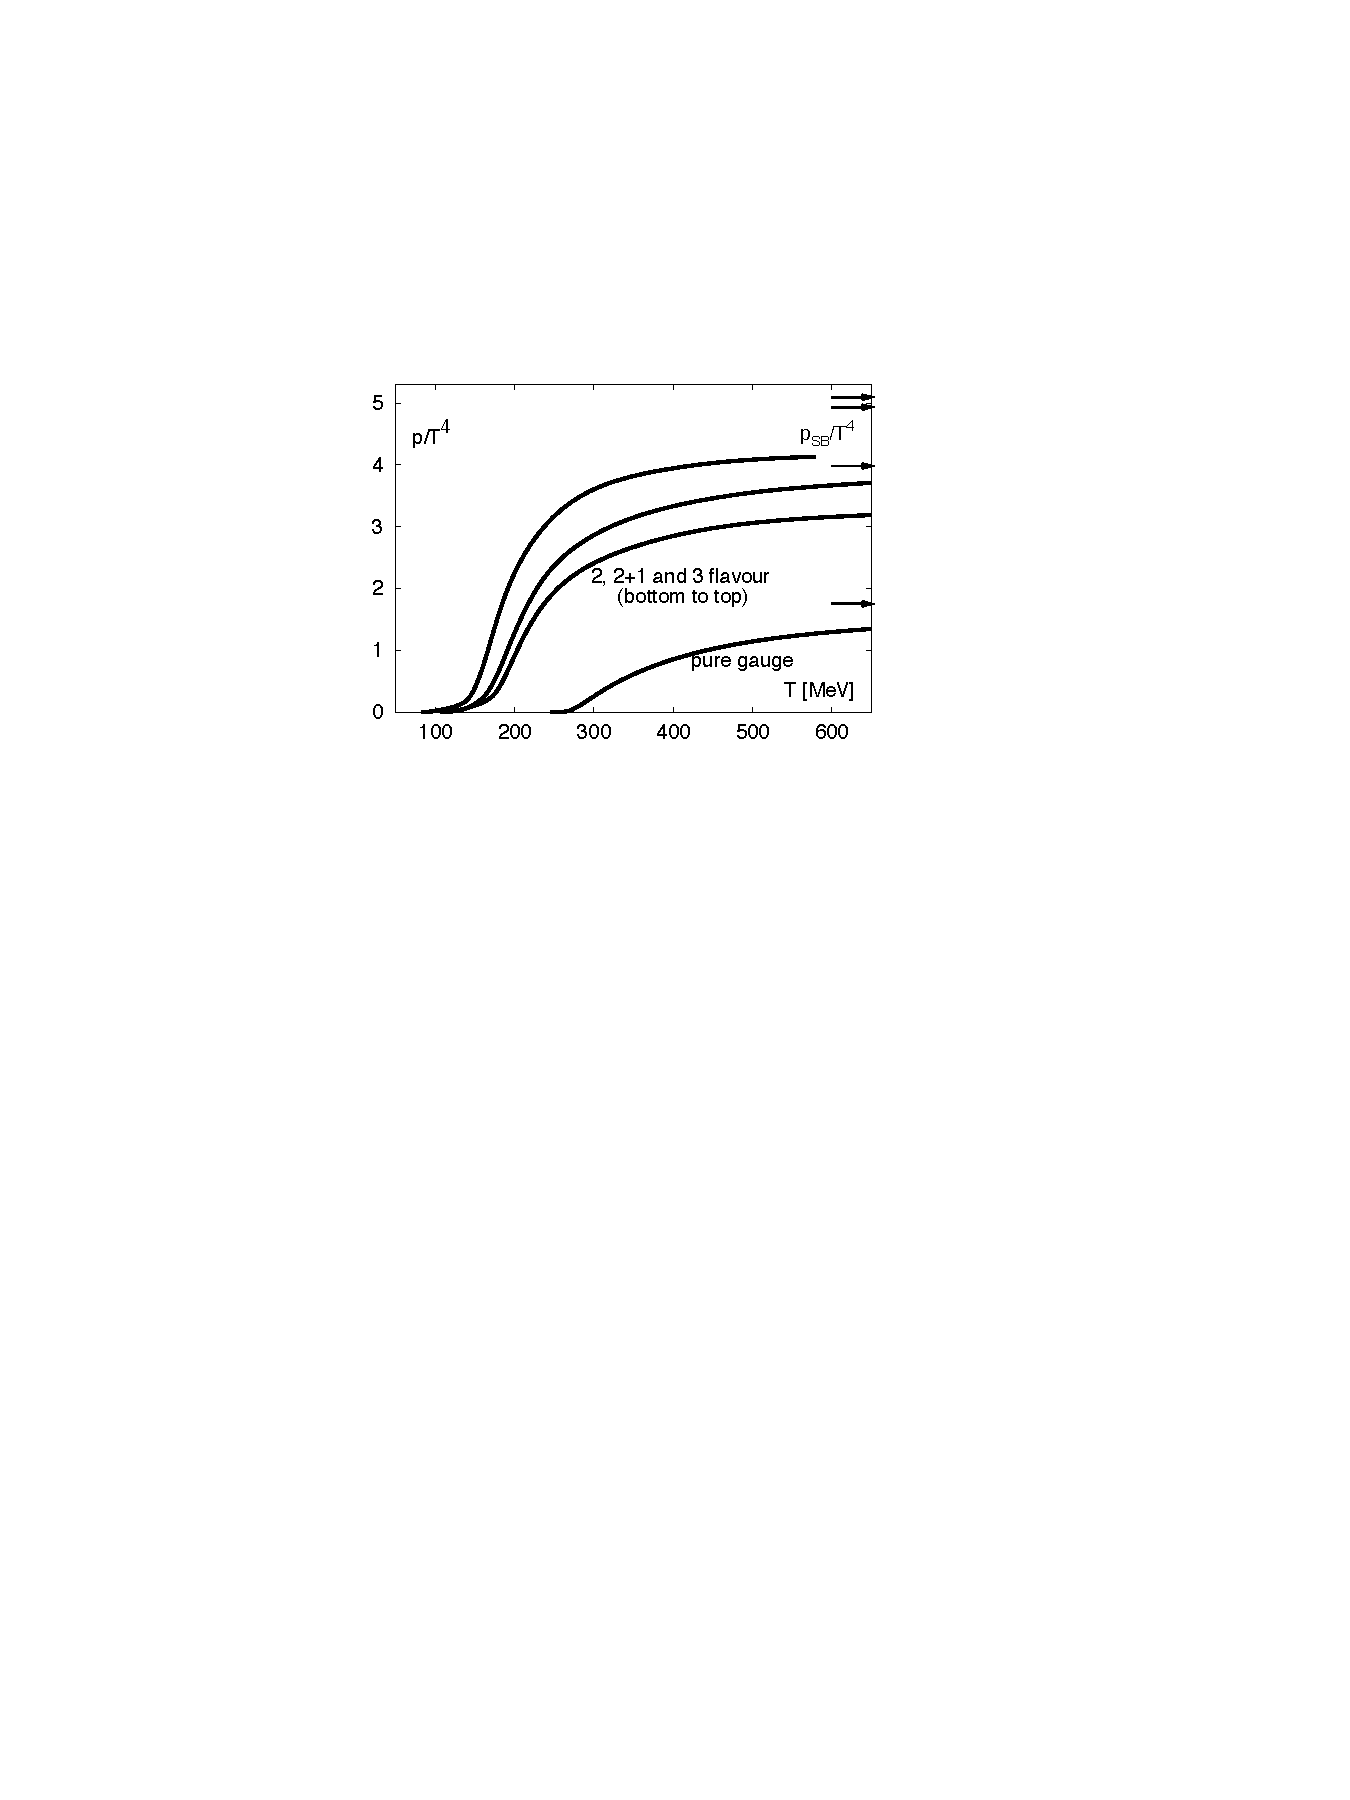
\includegraphics[scale=1.0]{Plots/Intro/pressure.pdf}
\end{center}
\caption[$p/T^4$ Calculations]{Calculations of $p/T^4$ in QCD for various numbers of quark flavors. Large jump near $T_c$ is the result of an increase in the number of degrees of freedom in the medium and is caused by the deconfinement of hadronic matter~\cite{hitempQCD}.}
\label{fig:pressure}
\end{figure}

\section{Experiments on QGP}

\subsection{Heavy Ion Collisions}

The prediction that deconfined matter could exist at sufficiently high temperatures and densities stimulated scientific interest in creating these conditions experimentally. The idea was to collide the nuclei of heavy elements at relativistic speeds, at high enough energy, these collisions could recreate the conditions in the Universe shortly after the Big Bang. The first generation of experiments looking for QGP were fixed target programs at the Alternating Gradient Synchrotron at Brookhaven National Laboratory and the Super Proton Synchrotron at CERN. Initial hints towards deconfinement were seen in these experiments. The WA97 and NA49 experiments observed large enhancement for strange baryons in Pb+Pb collsions which could be explained by a phase transition to a state with approximate strange quark equilibration.

The early fixed target results pointed in the direction of QGP but were not conclusive proof of its existence. The next step for QGP research was to move to collider based experiments. In 2000 the Relativistic Heavy Ion Collider (RHIC) began operating with the capability to collide gold nuclei at 200 GeV per nucleon center of mass energy, $\sqrt{s_{NN}}$. A decade later the Large Hadron Collider (LHC) began colliding lead nuclei at $\sqrt{s_{NN}}$ > 2 TeV. Key measurements have been made by the experiments at RHIC pointing towards the existence of a strongly interating deconfined phase of matter. We will now discuss some of these results which include: thermal production of light hadrons, elliptic flow of particles, and suppression of high $p_T$ particles and jets in central collisions. We will then look in particular at the measurements made in the heavy flavor sector (charm and bottom quarks) and motivate future observations there.

\subsection{Hadron Yields}

To look for signs of the QCD phase transition and the QGP, we want to study central collisions of heavy ions. In heavy ion collisions the two nuclei are offset from each other by some impact parameter, and thus their region of overlap is an ellipsoid. We refer to the degree of overlap between the colliding nuclei as the centrality and typically describe events by which percentile of centrality they fall into e.g. 10\%-20\% central (lower number corresponds to more central). The actual centrality definition is estimated based on models of the multiplicity observed in detector. The most central collisions have the largest and longest lived fireballs and thus create the most favorable conditions for producing QGP. 

One measurement to perform in heavy ion collisions is to measure the yields of hadrons from central collisions and compare them to thermal statistical models to extract the temperature and baryon chemical potential. Figure~\ref{fig:hadron_yields} shows the yields for several hadrons as measured by the experiments at RHIC along with the yields as determined by the fits to a thermal statistical model. From this the temperature at chemical freeze-out (the point in the evolution of the medium at which particle flavors are fixed) can be measured and it is calculated to be 164 MeV~\cite{thermstat}.

\begin{figure}[htbp]
\begin{center}
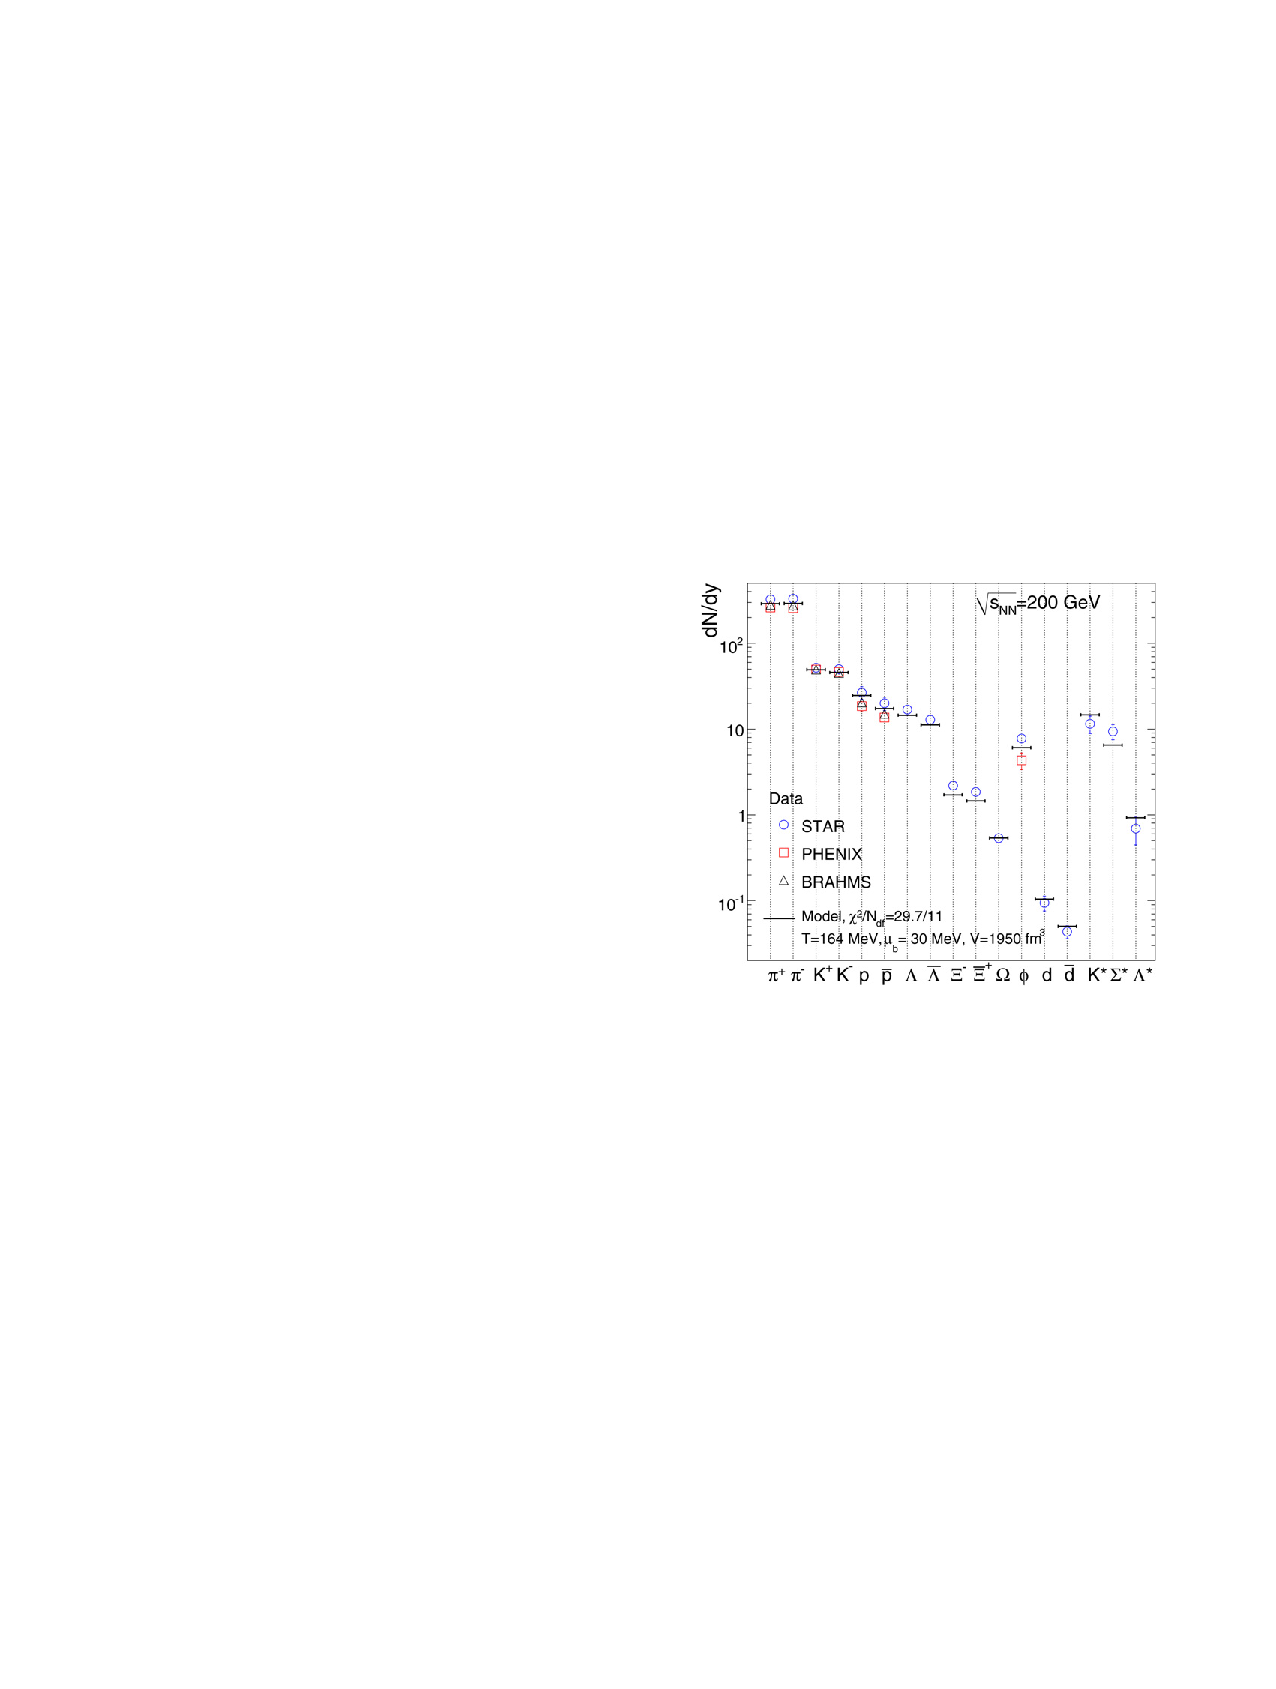
\includegraphics[scale=1.2]{Plots/Intro/had_yields.pdf}
\end{center}
\caption[Hadron Yields]{Yields for various hadrons in central collisions at RHIC energies compared to calculations from themal statistical models~\cite{thermstat}.}
\label{fig:hadron_yields}
\end{figure}

Comparisons can be made across several experiements with different collision energies to look for evidence of a phase transition. Figure~\ref{fig:T_mu} shows the T and $\mu_B$ extracted from the thermal statistical model fits as a function of the collision energy. The lower points come from the fixed target programs at the AGS and SPS while the highest data point corresponds to RHIC energies. The saturation temperature at chemical freeze-out around T $\sim$ 160 MeV as energy increases is indicative of the maximum temperature that hadronic matter may have.

\begin{figure}[htbp]
\begin{center}
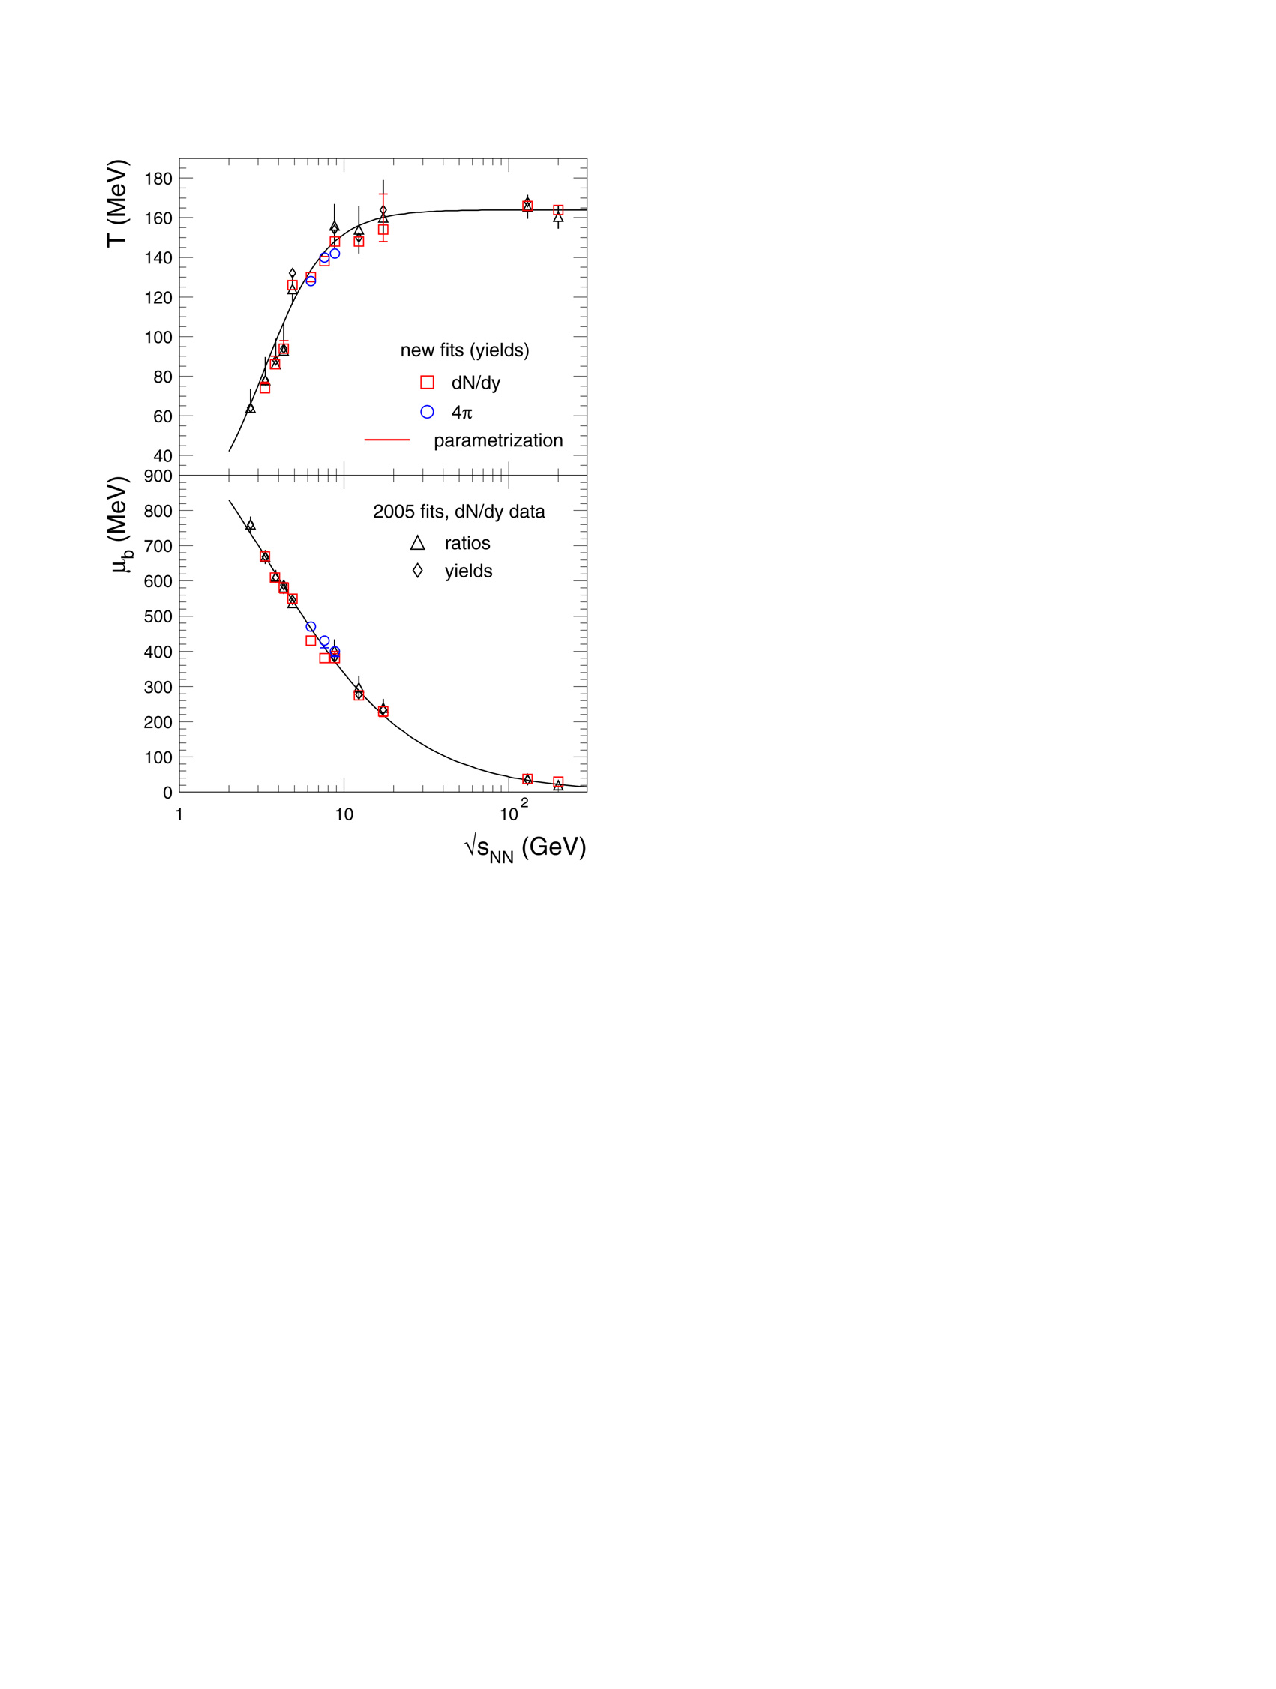
\includegraphics[scale=1.3]{Plots/Intro/freezeout.pdf}
\end{center}
\caption[Freeze-out T and $\mu_B$]{Temperature and baryon chemical potential extracted from thermal statistical model as a function of collision energy~\cite{thermstat}.}
\label{fig:T_mu}
\end{figure}

\subsection{Elliptic Flow}

In heavy ion collisions the nuclei do not exactly overlap, instead leaving an ellipsoidal region where temperatures and densities are high enough to create quark gluon plasma. This ellipsoidal overlap region creates an initial position space anisotropy which leaves an anisotropic pressure gradient along the fireball which manifests itself as an momentum dependent azimuthal anisotropy in the final state. More formally, the distribution of particles as a function of azimuthal angle can be written out as a Fourier expansion~\cite{v2long}:

\begin{equation}\label{eq:v2def}
E\frac{d^3N}{d^3p} = \frac{1}{2\pi}\frac{d^2N}{p_Tdp_Tdy}[1 + \sum_{n=1}^{\infty}2 v_n \cos(n(\phi - \Psi_r))]
\end{equation}

Where $\Psi_r$ is the angle of the reaction plane, which for our purposes can be thought of as the plane perpendicular to the major axis of the ellipsoid. The elliptic flow is the coefficient of the second term of this expansion, $v_2$. In Au+Au collisions at RHIC $v_2$ is large for light hadrons and consistent with hydrodynamic models at low $p_T$ ($\leq 2$ GeV/c), at higher $p_T$ the contribution of jets to $v_2$ needs to be considered. These measurements of $v_2$ point to a high degree of thermalization in collisions at RHIC energies and the mass dependence of $v_2$ indicates a collective flow of the medium.

An interesting extension for $v_2$ measurements is to look at how $v_2$ scales with the number of constituent quarks. To measure this experimentally, measurements of $v_2$ are performed for identified particles, then the results, scaled by the number of constituent quarks in the particle, are examined. Results for $v_2$ in 200 GeV Au+Au collisions in STAR scaled by number of constituent quarks are shown in Figure~\ref{fig:ncqscale}. From the plots we can see that the scaled $v_2$ in hadrons follows a universal trend for low $p_T$. This observation is consistent with the expectation for the main hadronization mechanism at low $p_T$ to be coalescence of quarks and that in the collective evolution of the medium the partonic, rather than hadronic, degrees of freedom are most relevant~\cite{ncqscale}. 

\begin{figure}[htbp]
\begin{center}
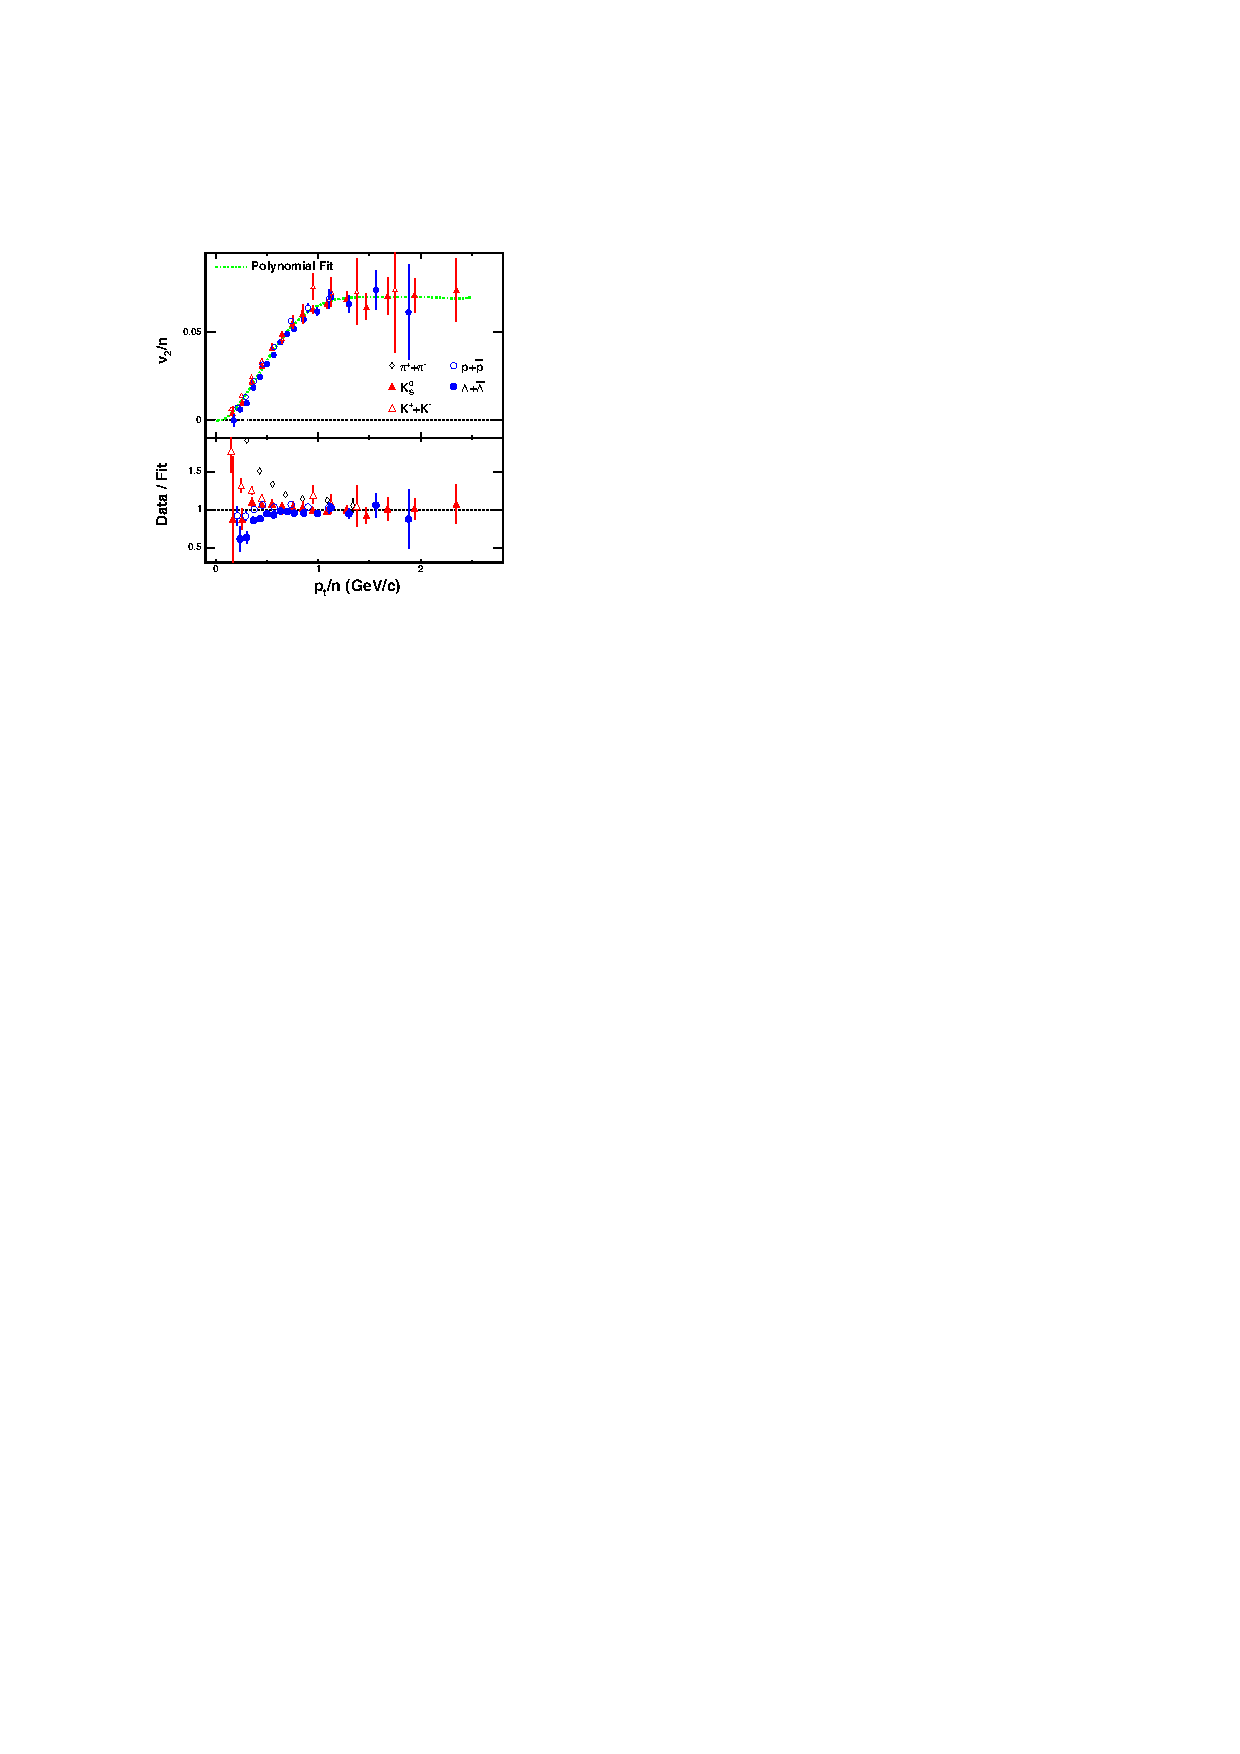
\includegraphics[scale=1.7]{Plots/Intro/ncq_scale.pdf}
\end{center}
\caption[NCQ Scaling of $v_2$]{Identified particle $v_2$ as measured in 200 GeV Au+Au minimum bias collisions in STAR scaled by the number of constituent quarks. Common trend across hadrons is evidence for hadronization from coalescence of thermalized quarks~\cite{ncqscale}.}
\label{fig:ncqscale}
\end{figure}

\subsection{$R_{AA}$ and Jet Suppression}

Another technique for studying QGP is to compare observables between heavy ion collisions and p+p data. In proton-proton collisons on average the degree of collective motion of the nuclear medium is expected to be small and can be used as a baseline reference. Here we will explore two different ways of comparing heavy ion and p+p systems. The first is the nuclear modification factor which compares particle yields in  heavy ion systems to the scaled up yields from p+p, differences in theses yields could be signs of further interactions with the medium. We will also look at jet modification. Jets are the product of hard scattering of quarks and gluons in the initial collision, as a hard quarks traverses the QGP it will be subjected to strong interactions with the medium and lose energy. The suppression of high $p_T$ jets is further evidence for the existence of QGP.

In collider experiements, high $p_T$ particles are generated from the initial hard scattering of partons in the collisions. Without any sort of medium effects from QGP we could model the collision of two heavy nuclei as a superposition of independent binary proton collisions. Deviation from this behavior indicates extra effects from the medium. We can also investigate and control for the effects of cold nuclear matter by studying modification of yields in d+Au collisions. We define the ratio of yields in heavy ion to scaled p+p as the nuclear modification factor $R_{AA}$. Which is explicitly defined as:

\begin{equation}\label{eq:RAAdef}
R_{AA}(p_T) = \frac{(1/N_{AA}) d^2N_{AA}/dp_Tdy}{\langle N_{coll} \rangle/\sigma^{incl}_{pp}(d^2\sigma_{pp}/dp_Tdy)} 
\end{equation}

where $ \langle N_{coll} \rangle $ is the average number of collisions as calculated by a Glauber model simulation. Figure~\ref{fig:piRAA} shows the measurement of $\pi^0$ $ R_{AA}$ in Au+Au collisions in PHENIX. In central collisions, where we expect QGP formation and jet medium interactions, the yield is highly suppressed at high transverse momentum. In the peripheral bin where no QGP is expected to be formed the $R_{AA}$ is consistent with 1, meaning the yields are what would be expected from a superposition of p+p collisions. Moving from most central to most peripheral bins, the yields gradually go from highly suppressed to not supressed at all, as we would expect since the more central bins produce regions of higher temperature and density increasing the jet-medium interaction.

\begin{figure}[htbp]
\begin{center}
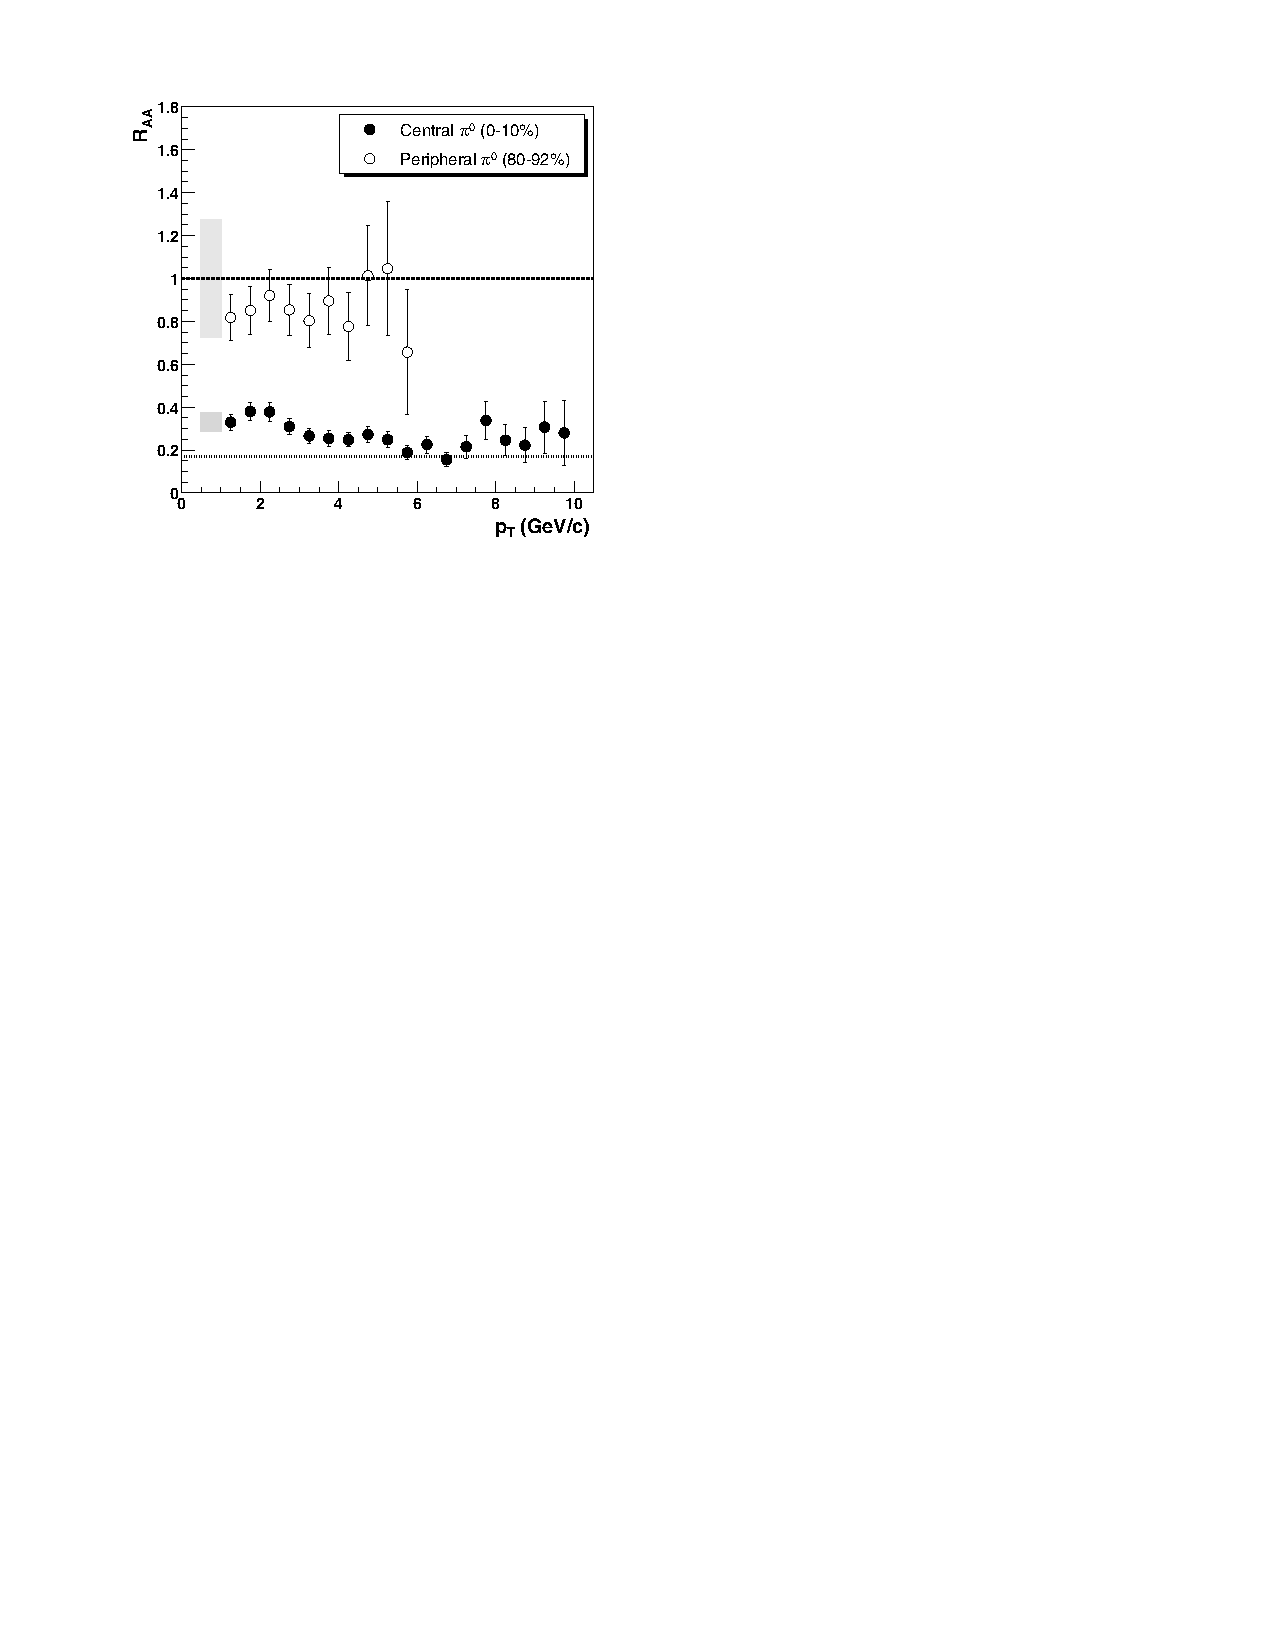
\includegraphics[scale=1.2]{Plots/Intro/pi_RAA.pdf}
\end{center}
\caption[$R_{AA}$ for $\pi^0$]{PHENIX measurement of $R_{AA}$ for $\pi^0$ in central and peripheral Au+Au collisions. Large suppression of yields is seen in central collisions~\cite{PHENIXpiRAA}.}
\label{fig:piRAA}
\end{figure}

The properties of the QGP can also be probed by examining the effects on high $p_T$ partons as they traverse the medium. The high $p_T$ light quarks are created by hard processes early in the collision and are theorized to lose energy due to induced gluon radiation in the QGP. The energy loss leaves softer particles in jets and the broadening of spatial jet-like correlations. STAR investigated light flavor jet correlations by looking at azimuthal correlations of particles in Au+Au, p+p, and d+Au collisions. High $p_T$ particles were used as the leading particles and correlated with other hadrons in the event.

\begin{figure}[htbp]
\begin{center}
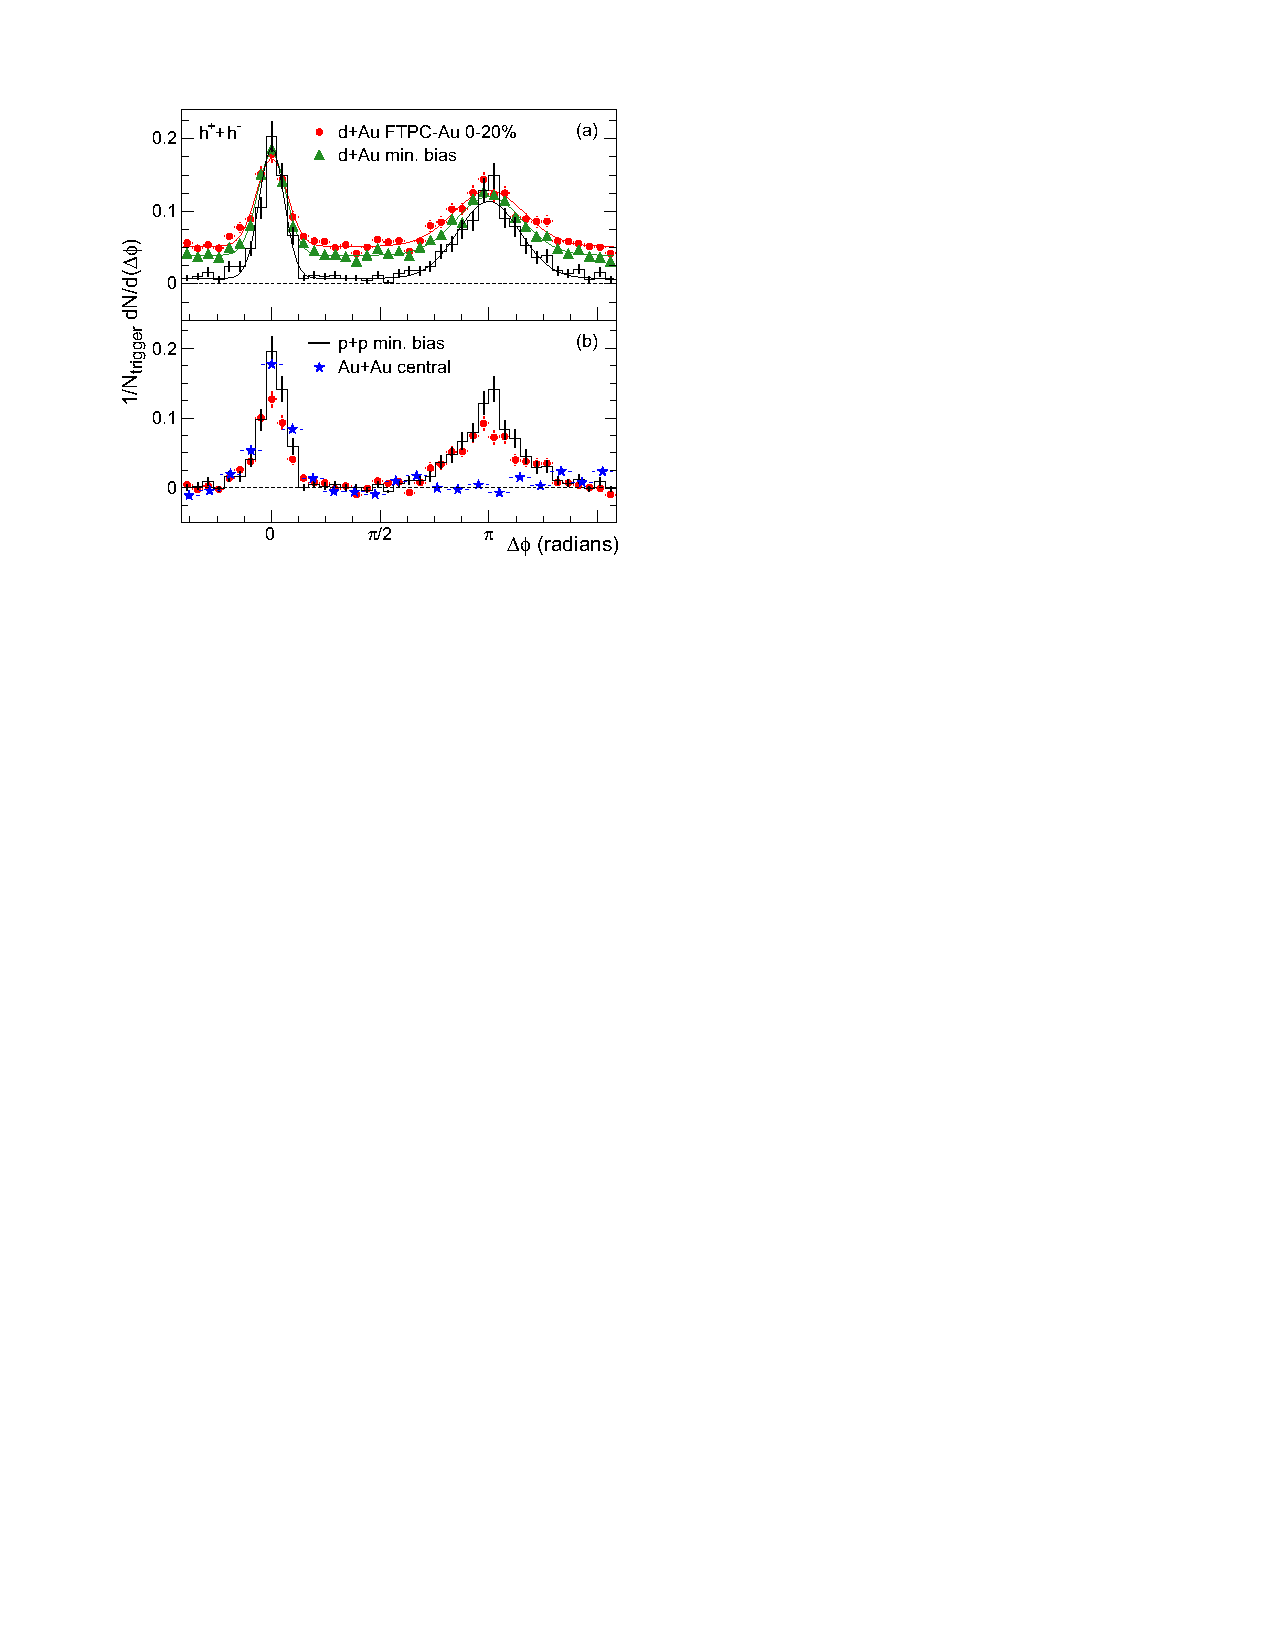
\includegraphics[scale=1.2]{Plots/Intro/jet_quench.pdf}
\end{center}
\caption[Jet Quenching is STAR]{Azimuthal dihadron correlations in STAR. Strong quenching of the away side jet is seen in Au+Au collisions but not p+p or d+Au. Lack of suppression in d+Au rules out cold nuclear matter effects on jet suppression~\cite{STARdihad}.}
\label{fig:jet_quench}
\end{figure}

Figure~\ref{fig:jet_quench} shows the azimuthal dihadron correlations measured in STAR. In p+p and d+Au we see strong back-to-back correlations of particles due to momentum conservation in the initial production of hard partons. The consistency of p+p and d+Au correlations is evidence that there is little interaction between the jets and the medium in these collisions. The slight broadening and enhanced yields in the away side are consistent with expectations from pQCD models with the Cronin effect~\cite{cronin}. However, in Au+Au the away side jet is strongly suppressed, indicating that light quarks lose a substantial amount of energy within the hot and dense medium created in heavy ion collisions leading to reduced yields of high $p_T$ associated particles in central Au+Au events.

\section{Heavy Flavor Probes}

\subsection{Motivation}

The observables discused so far have been largely concerned with phenomena involving the light quarks ($u$ and $d$) which have different sensitivity to the evolution of the QGP than heavy quarks. Thermal production and coallesence of light quarks into hadrons as well as collectivity of light quarks are evidence for a hot dense strongly interacting QCD matter being produced in heavy ion collisions. Heavy quarks can also be used to probe the QGP and help illuminate additional properties of the medium that are harder to explore with light flavor observables. 

Heavy flavor quarks, by which we mean charm ($c$) and bottom ($b$) quarks, are an important additional avenue of study in heavy ion physics for a few reasons. The light quarks have masses $\sim2-6$ MeV/$c^2$ while the heavy flavor quarks have masses $\sim1.3$ GeV/$c^2$ for charm and $\sim4.3$ GeV/$c^2$ for bottom. Unlike the light quarks the masses of the heavy quarks are well above the temperatures found in the medium produced by relativistic heavy ion collisions. This means that thermal production, which often complicates light flavor analyses, does not need to be considered for heavy flavor. Instead heavy flavor is exclusively produced by hard processes in the very early stages of the collision. Thus heavy quark observables will be sensitive the entire evolution of the medium. Also the energy scale for heavy quark production is high enough ($M_{c,b} \gg \Lambda_{QCD}$) that the production can be accurately described with pQCD.

The energy loss of heavy quarks in QGP is also an area of significant interest. Earlier we discussed jet quenching as a result of light flavor quarks losing energy in a strongly interacting medium. The mechanism behind light quark energy loss in the QGP is theorized to be induced gluon radiation, and when calculating the radiative energy loss it can be assumed that the light quarks are massless. In the propagation of heavy flavor quarks this assumption cannot be made. Instead for heavy quarks the radiative energy loss differs from the massless case by a factor:

\begin{equation}\label{eq:deadcone}
\Big( 1 + \frac{\theta^2_0}{\theta^2} \Big)^{-2}
\end{equation}

where $ \theta_0 = \frac{m}{E}$~\cite{glurad}. This means that relative to light flavor, the gluon radiation from heavy flavor quarks is suppressed at small angles $\theta$. This phenomenon is known as the `dead cone effect". Instead, in the heavy flavor sector, it's possible that collisional losses from elastic scattering in the medium plays a much more significant role.

\subsection{Experimental Results}

While heavy flavor observables are of considerable interest in the study of QGP they come with some serious complications compared to the light flavor obeservables. Production rates for charm and bottom are lower and thus many heavy flavor measurements are limited by statistics. Only in the last several years has RHIC produced high statistics Au+Au data sets opening up studies in heavy flavor. Another problem is that the heavy quarks mostly hadronize into $D$ and $B$ mesons which are short lived and it is difficult to reconstruct these decays with high efficiency, especially in heavy ion collisions. Since 2014 STAR has installed the Heavy Flavor Tracker to improve secondary vertex resolution and allow better reconstruction of heavy flavor decays. An alternative to direct reconstruction of $D$ or $B$ is to look only at the electrons produced from semi-leptonic decays of these mesons. At high $p_T$ ($> 2$ GeV/c) the direction of a decay daughter electron is well correlated with the parent meson, these electrons can then be used as a proxy for the $D$ or $B$ meson. The branching ratios for semi-leptonic decays of heavy flavor mesons is on the order of 10\%~\cite{pdg} which further limits the possible statistics.

\begin{figure}[htbp]
\begin{center}
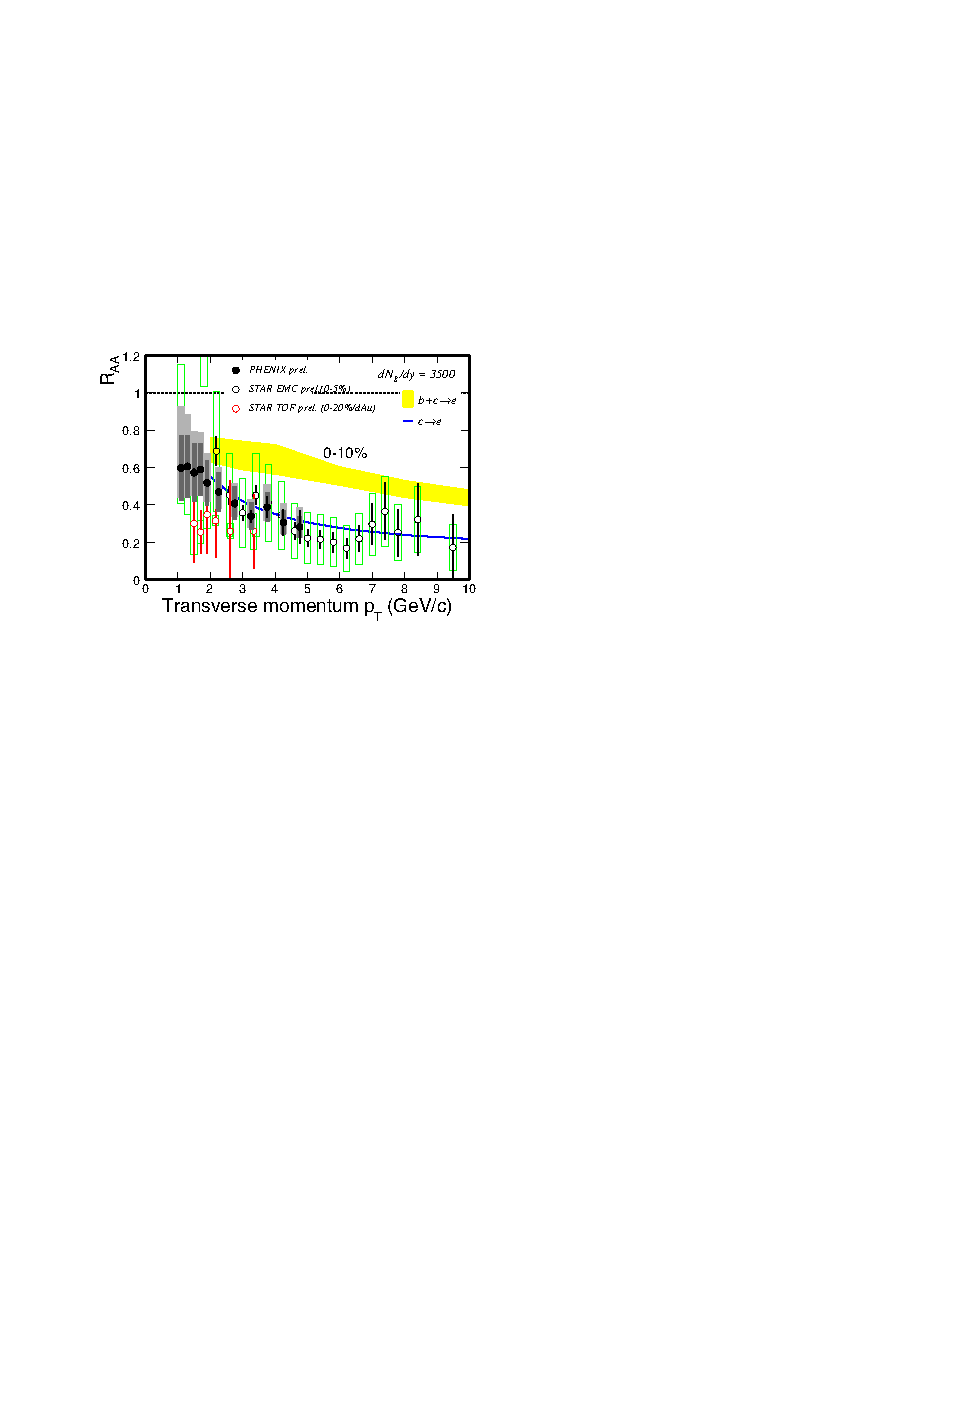
\includegraphics[scale=1.8]{Plots/Intro/hf_raa.pdf}
\end{center}
\caption[NPE $R_{AA}$]{Non-photonic electron $R_{AA}$ from central Au+Au collisions measured by STAR and PHENIX. The theoretical curves show expected suppression due to radiative energy loss. The measured $R_{AA}$ is consistent with measurements of light flavor $R_{AA}$~\cite{NPERAA}.}
\label{fig:hf_raa}
\end{figure}

Like in light flavor we can measure the $R_{AA}$ for heavy flavor to look for effects of the medium relative to p+p systems. If we considered that the induced gluon radiation from heavy quarks is reduced at low angles, then we might expect to see a higher $R_{AA}$ (less suppression of yield relative to superposition of binary collisions) in heavy flavor. STAR and PHENIX have measured $R_{AA}$ for electrons from semi-leptonic $D$ and $B$ decays. The results are summarized in Figure~\ref{fig:hf_raa}. Both experiments see values of $R_{AA}$ around $.2-.3$ at high $p_T$ which is consistent with the suppression of yields observed in light flavor hadrons.

The theoretical curves show the predictions of suppression due to radiative energy loss for decays from $c$ as well as $c$ and $b$ combined. It is difficult to explain the large suppression for heavy flavor quarks if it is soley due to gluon radiation. Models which include collisional energy loss for heavy quarks as well predict a larger suppression.

\begin{figure}[htbp]
\begin{center}
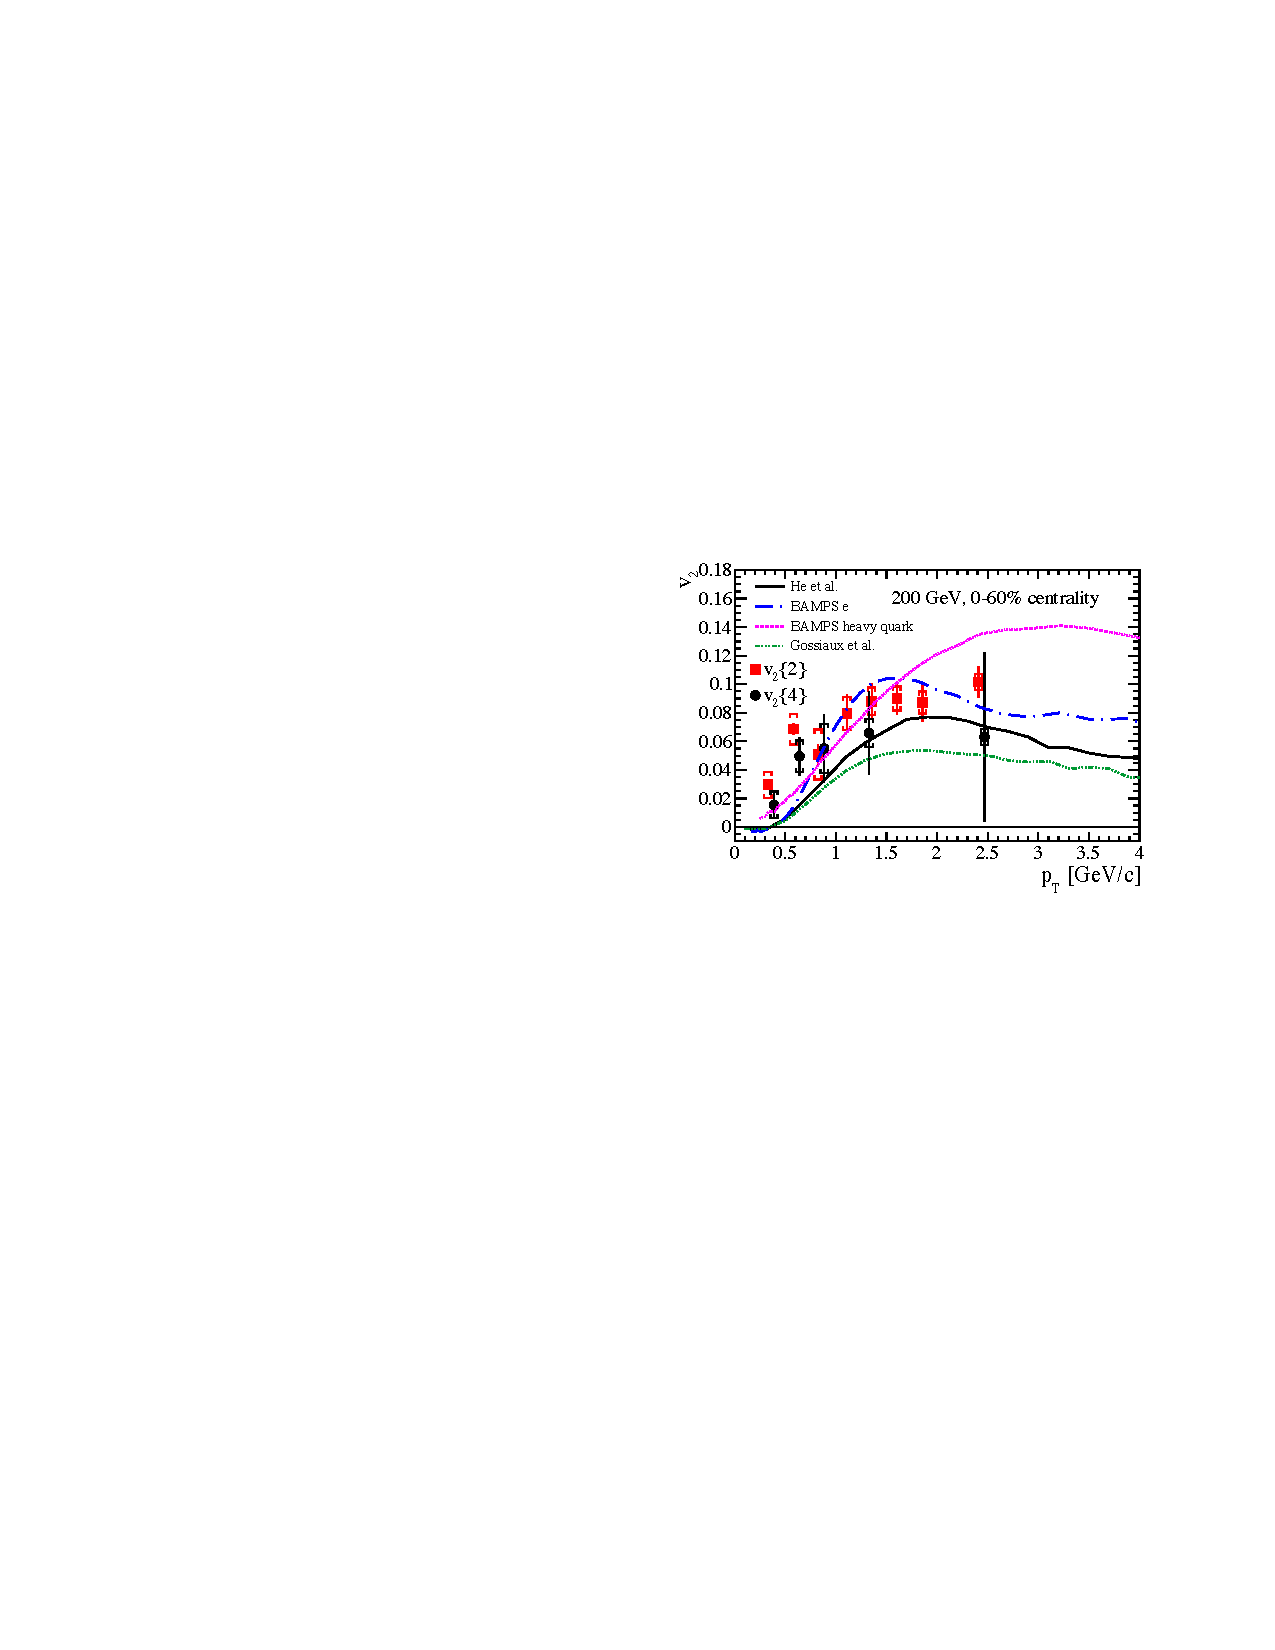
\includegraphics[scale=1.5]{Plots/Intro/npe_v2.pdf}
\end{center}
\caption[NPE $v_2$]{Elliptic flow of electrons from heavy flavor decays measured in STAR as well as predictions of $v_2$ relative to the reaction plane for various models~\cite{musNPEv2}.}
\label{fig:npe_v2_intro}
\end{figure}

Likewise elliptic flow in heavy flavor is also a subject of active study. The low $p_T$ $v_2$ can be used to study how thermalized $c$ and $b$ quarks are in the medium. Preliminary STAR measurements of $v_2$ for heavy flavor decay electrons are shown in Figure~\ref{fig:npe_v2_intro}, also included are theoretical predictions for various energy loss models for heavy quarks. The electron $v_2$ measurement is complicated by contributions from nonflow effects. A heavy quark traversing the medium will see different path lengths if it is in-plane versus out-of-plane. Path length dependence of jet modification for heavy flavor quarks could then contribute to $v_2$ separately from thermalization and collectivity. Non-flow effects are expected to be more prominent at high $p_T$.

\section{Heavy Flavor Two Particle Correlations}

While most analyses in the heavy flavor sector have focused on spectra, $R_{AA}$, and flow measurements, two particle correlations are also an important tool for studying the dynamics of heavy quarks. Two particle azimuthal correlations in light flavor were the tool for jet suppression measurements which were shown previously (Figure~\ref{fig:jet_quench}) and we hope to extend these measurements to the heavy flavor sector. The correlations rely on the fact that in the leading order of QCD processes, collisions of partons result in back-to-back pairs of dijets due to conservation of momentum. The modification of the resulting back-to-back correlations in the presence of QGP can be used to explore the interactions of quarks and the medium. Figure~\ref{fig:qqcorr} shows a theoretical calculation of the back-to-back correlations of heavy quarks produced in Pb+Pb collisions at LHC energies~\cite{qqazi}. We can see a few of the general modifications to the correlation that may arise from interactions with the medium. There is a difference depending on the energy loss model used, either purely collisional or collisional plus radiative. We also see that higher momentum pairs retain their initial back-to-back correlation more. It has also been suggested that for low momentum pairs the correlation may be enhanced on the near side due to the ``partonic wind"~\cite{partwind}.

\begin{figure}[htbp]
	\begin{center}
    \begin{subfigure}{0.75\textwidth}
        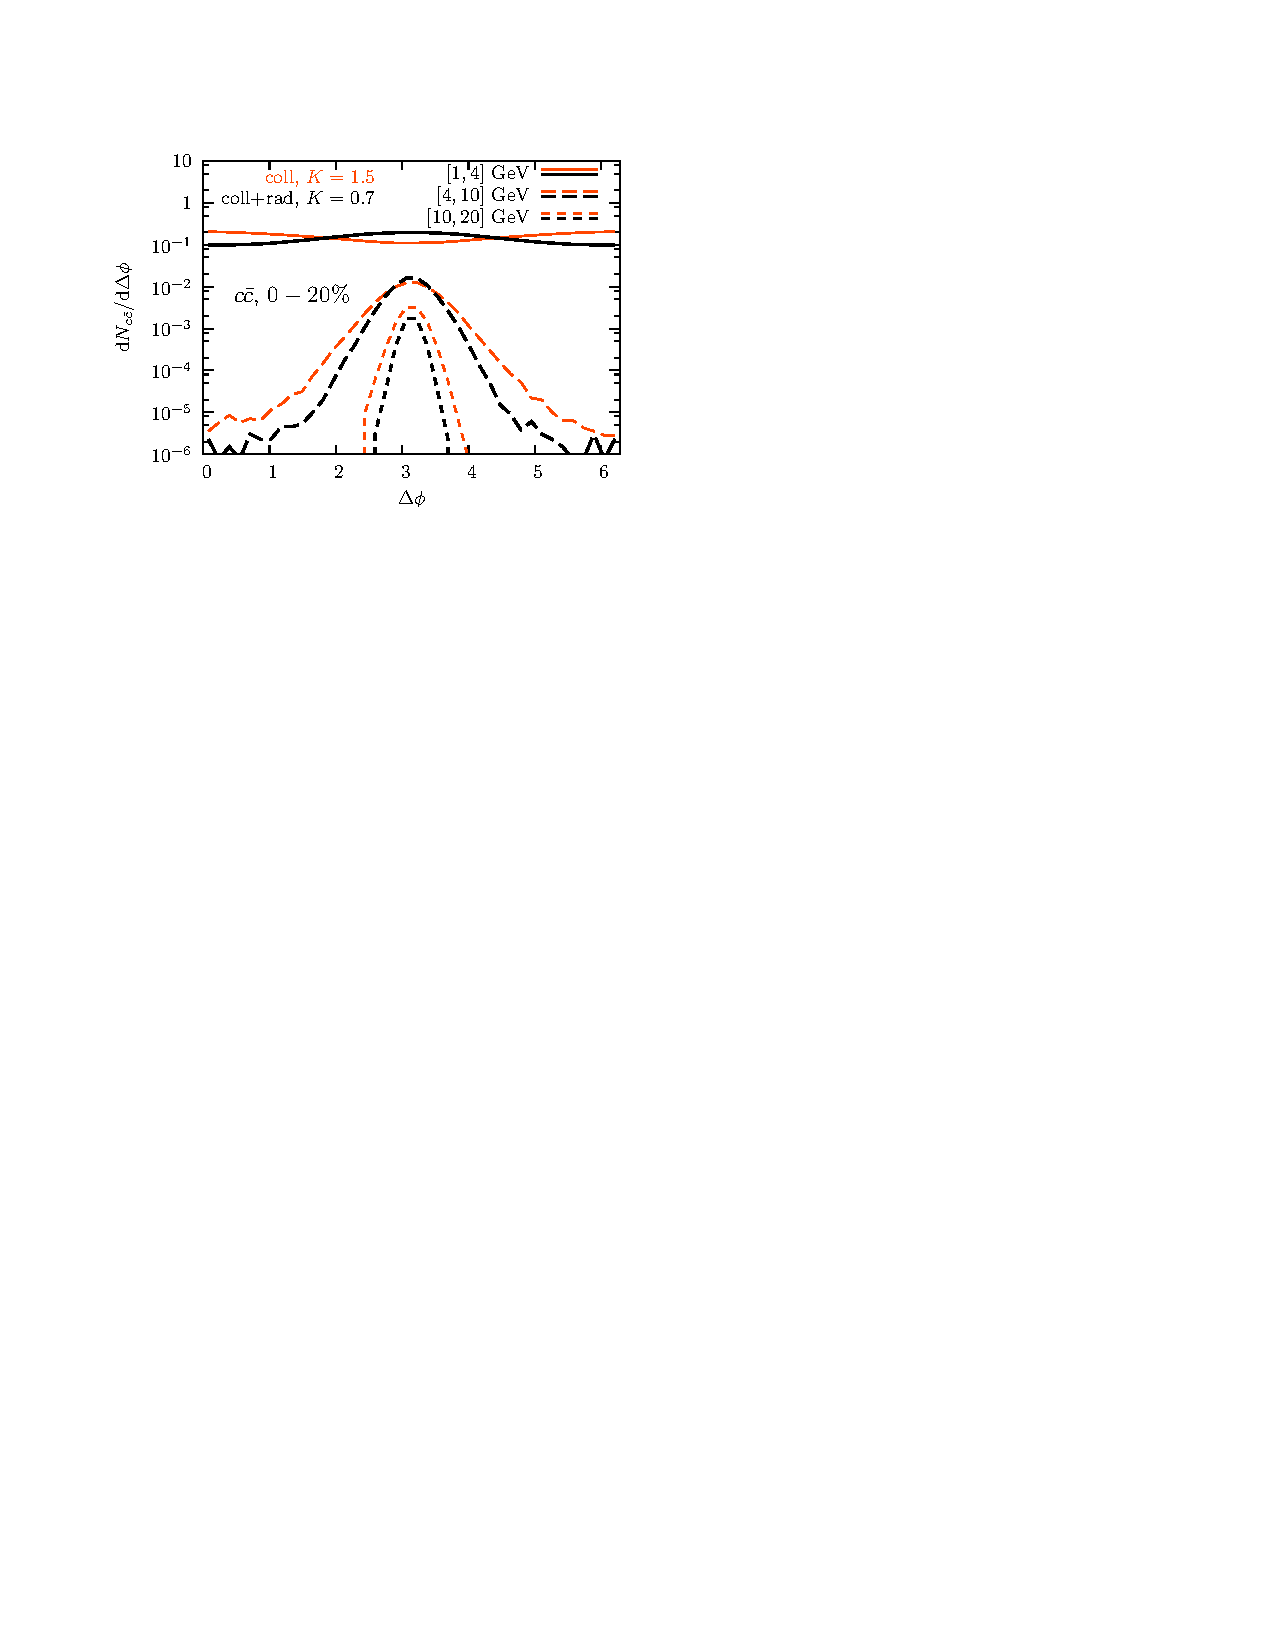
\includegraphics[width=\textwidth]{Plots/Intro/cc_cent.pdf}
        \caption{}
        \label{fig:ccbarcent}
    \end{subfigure}
    \begin{subfigure}{0.75\textwidth}
        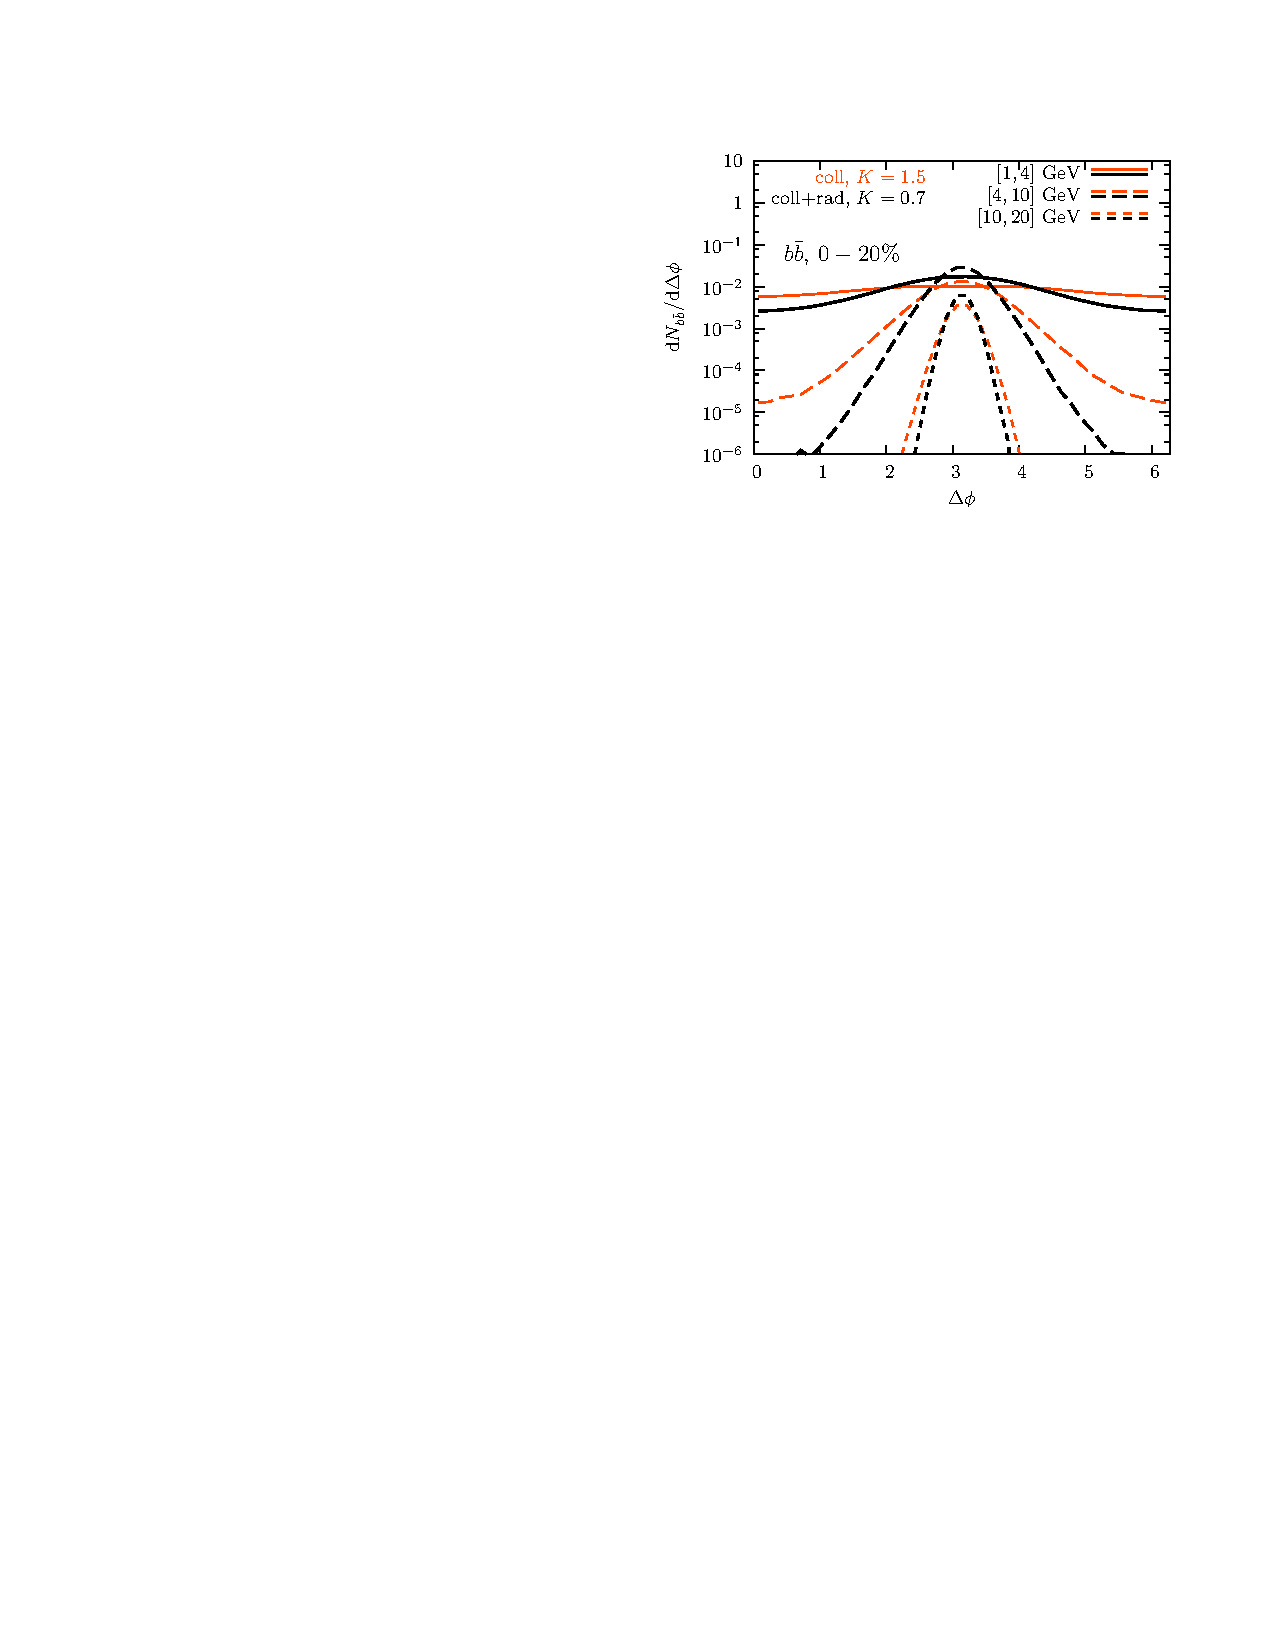
\includegraphics[width=\textwidth]{Plots/Intro/bb_cent.pdf}
        \caption{}
        \label{fig:bbbarcent}
    \end{subfigure}
	\end{center}
\caption[Correlations $c$ and $b$ at LHC Energies]{Theoretical calculations of azimuthal correlations for heavy quarks in Pb+Pb collisions at LHC energies. Differences in the models for energy loss can be seen as well as the dependence on $p_{T}$~\cite{qqazi}.}
\label{fig:qqcorr}
\end{figure}

In central collisions the two particle correlations showed a double peaked structure on the away side, this was possibly thought to be Mach cones, shockwaves in the QGP produced by the quarks, but it is more likely to be a correlation from triangular flow $v_3$. The energy loss of a quark passing through the QGP and losing energy due to induced gluon radiation is proportional to the product $\hat{q}L^2$. Here $\hat{q}$ is the transport coefficient, defined as the mean momentum spread per unit length traversed and from previous measurements is thought to be on the order of 10 $\text{GeV}^2/\text{fm}$. Two particle correlations can be used to explore the path length dependence of energy loss as the near side trigger jet may traverse through a shorter path in the QGP than the away side jet. However care must be taken as there is potentially bias a trigger towards emissions from the surface of the medium when looking at triggered two particle correlations~\cite{biasshower}. 

Heavy flavor two particle correlations look at the path length dependence of energy loss for heavy quarks and the relative contribution of radiative and collisional energy loss mechanisms. Ideally we would like to study the energy loss of the heavy quarks or the heavy flavor mesons directly, however this is not within the capabilities of current experiments. Instead we will need to rely on the electrons from semileptonic decays of $B$ and $D$ mesons. Figure~\ref{fig:two_part} shows a cartoon of how two particle correlations can investigate the dynamics of heavy quarks in QGP. A sufficiently high $p_T$ electron is used as the trigger particle in the correlation. The near side and away side of the correlation contain information on the decay products from the heavy mesons. We are also interested in the response of the medium to the quarks.

\begin{figure}[htbp]
\begin{center}
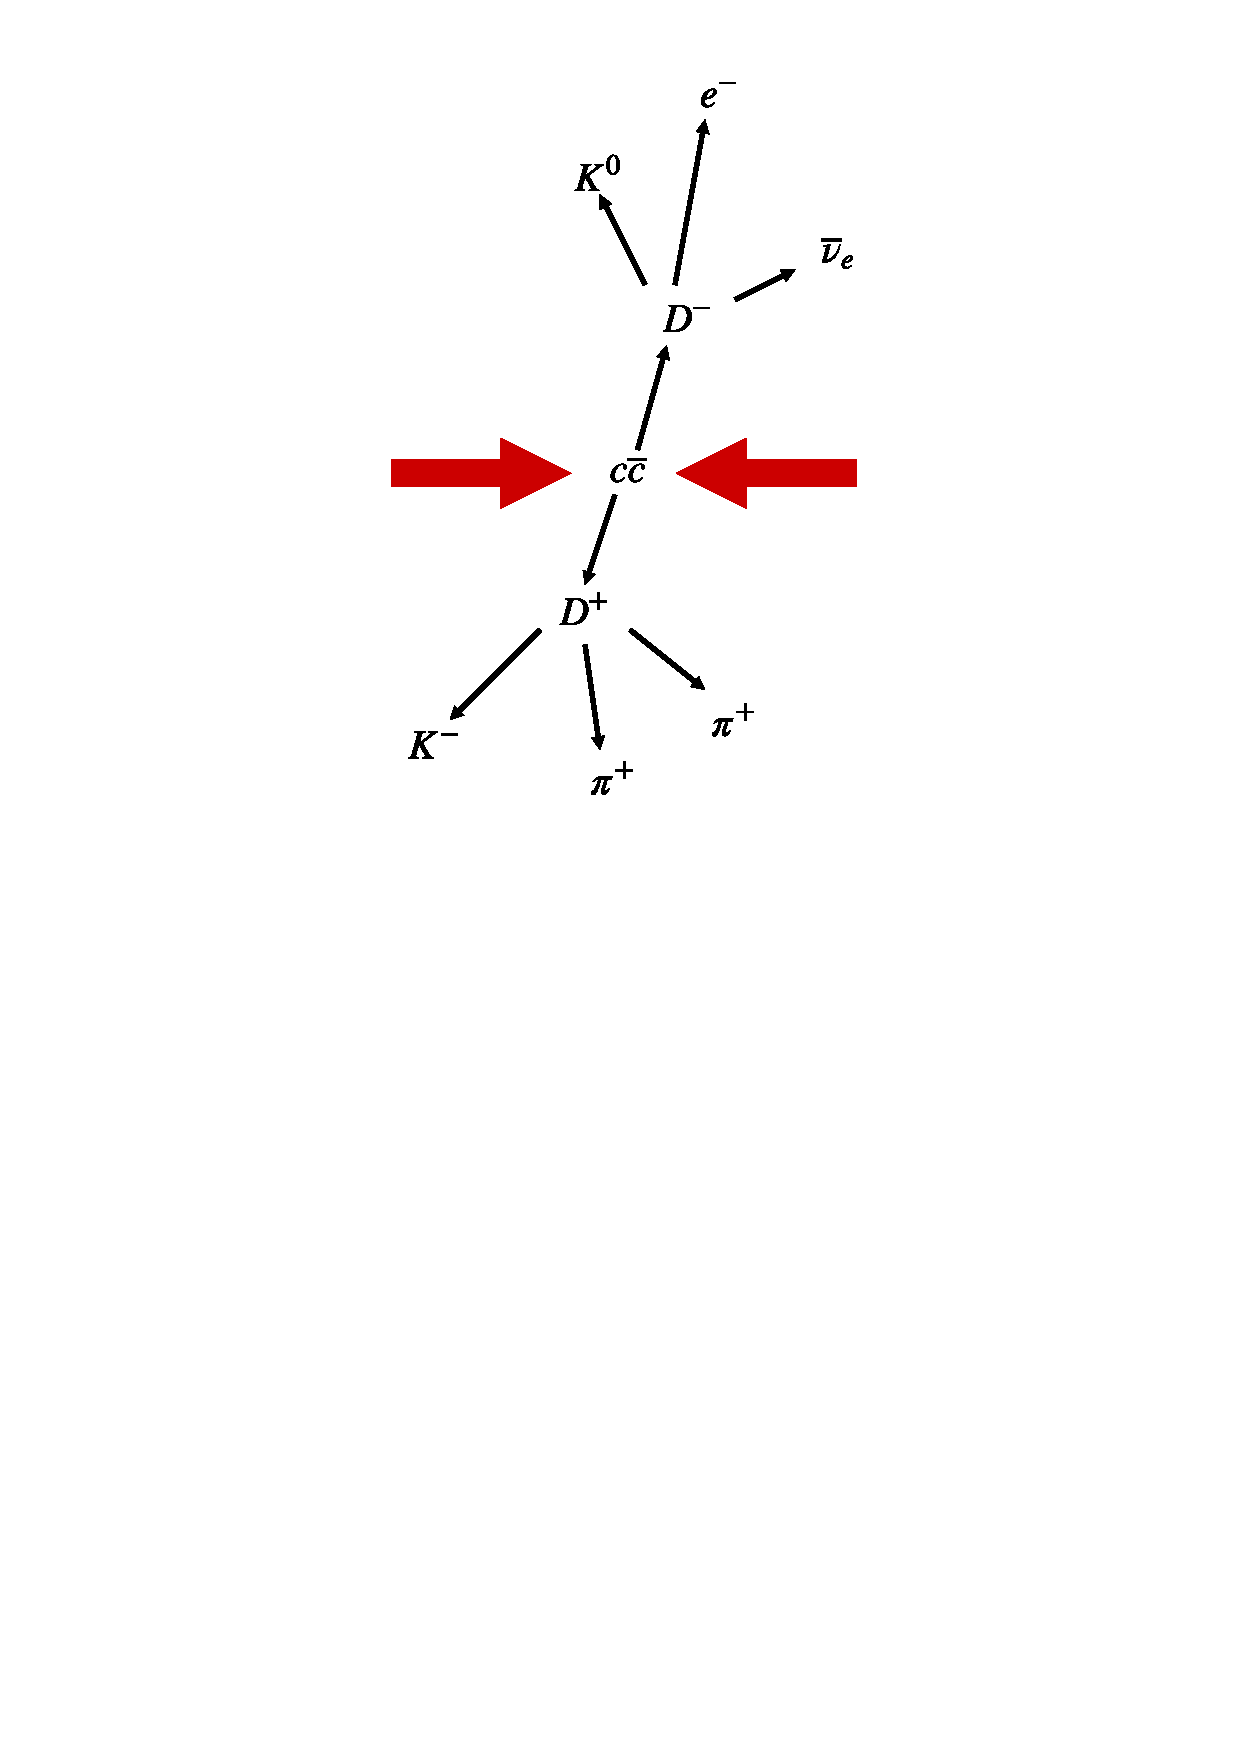
\includegraphics[scale=1.3]{Plots/Intro/ccbar.pdf}
\end{center}
\caption[Two Particle Correlation from $c\bar{c}$]{Illustration of two particle correlation coming from a produced $c\bar{c}$ pair. This diagram only shows the particles from the decays of heavy mesons but we are also interested in the effect of the heavy quarks on the medium as well.}
\label{fig:two_part}
\end{figure}

One of the largest challenges in constructing two particle correlations is limited statistics. STAR has previously looked at heavy flavor electron-hadron correlations to study the charm to bottom fraction produced in p+p collision~\cite{STARBDrat}. PHENIX has also measured correlations of electrons from heavy flavor decays (Figure~\ref{fig:phenix_eh}) in both p+p and Au+Au~\cite{PHENIXeh}. In 2010 and 2011 RHIC completed high statistics Au+Au runs opening up the possibility of much improved measurements of heavy flavor two particle correlations. This dissertation will focus on constructing two particle correlations between electrons from heavy flavor decays (here called \textit{nonphotonic electrons}) and hadrons. The chapters will cover the experimental apparatus, the procedure for identifying electrons, and then making correlations themselves as well as calculating backgrounds. The physics implications of e-h correlations will also be discussed. 

\begin{figure}[htbp]
\begin{center}
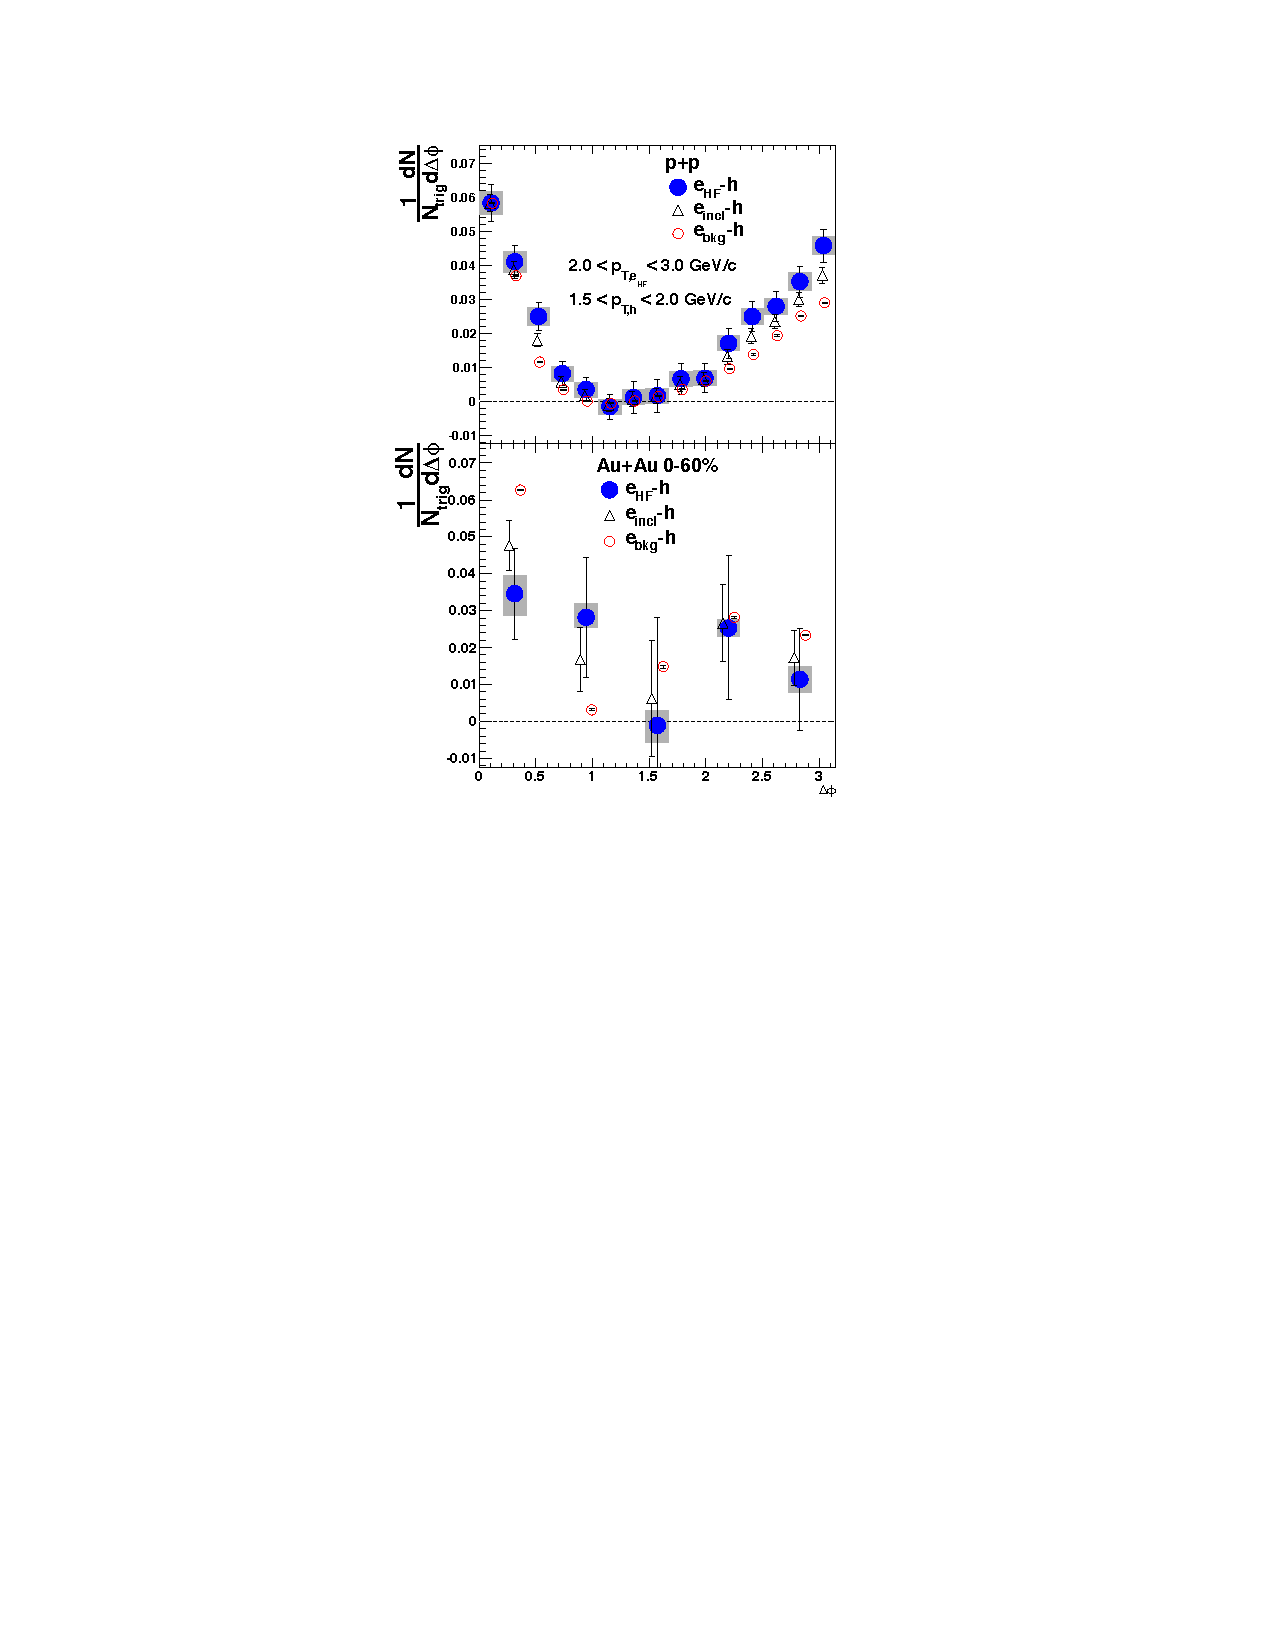
\includegraphics[scale=1.3]{Plots/Intro/phenix_eh.pdf}
\end{center}
\caption[PHENIX e-h correlation]{Azimuthal correlation of electrons from heavy flavor decays to hadrons in p+p and Au+Au as measured by PHENIX~\cite{PHENIXeh}.}
\label{fig:phenix_eh}
\end{figure}
